\documentclass[12pt,a4paper]{article}

% ------------------- Paquetes -------------------
\usepackage[utf8]{inputenc}
\usepackage[spanish]{babel}
\usepackage{amsmath,amssymb,amsthm}
\usepackage{graphicx}
\usepackage{hyperref}
\usepackage{booktabs}
\usepackage{geometry}
\usepackage{setspace}
\usepackage{natbib}
\usepackage{listings}
\usepackage{xcolor}
\usepackage{enumitem}
\usepackage{caption}
\usepackage{subcaption}
\usepackage{fancyhdr}
\usepackage{titlesec}
\usepackage{float}
\usepackage{colortbl}
\usepackage{multirow}
\usepackage{longtable}
\usepackage{algorithm}
\usepackage{algpseudocode}
\usepackage{amsmath}

% Teoremas y definiciones
\newtheorem{definition}{Definición}[section]
\newtheorem{theorem}{Teorema}[section]

% ------------------- Configuración -------------------
\geometry{margin=2.5cm}
\onehalfspacing

\definecolor{codegreen}{rgb}{0,0.6,0}
\definecolor{codegray}{rgb}{0.5,0.5,0.5}
\definecolor{codepurple}{rgb}{0.58,0,0.82}
\definecolor{backcolour}{rgb}{0.95,0.95,0.92}

\lstdefinestyle{mystyle}{
    backgroundcolor=\color{backcolour},
    commentstyle=\color{codegreen},
    keywordstyle=\color{magenta},
    numberstyle=\tiny\color{codegray},
    stringstyle=\color{codepurple},
    basicstyle=\footnotesize\ttfamily,
    breakatwhitespace=false,
    breaklines=true,
    captionpos=b,
    keepspaces=true,
    numbers=left,
    numbersep=5pt,
    showspaces=false,
    showstringspaces=false,
    showtabs=false,
    tabsize=4
}
\lstset{style=mystyle}

\hypersetup{
    colorlinks=true,
    linkcolor=blue,
    citecolor=blue,
    urlcolor=blue
}

% ------------------- Encabezados -------------------
\pagestyle{fancy}
\fancyhf{}
\fancyhead[L]{\leftmark}
\fancyhead[R]{\thepage}
\fancyfoot[C]{\thepage}

% ------------------- Portada -------------------
\title{
    \vspace{2cm}
    \Huge\textbf{Buscaminas Inteligente:}\\[0.4cm]
    \Large\textbf{Modelado, Resolución y Visualización del Juego Buscaminas}\\[0.2cm]
    \Large\textbf{mediante Teoría de Grafos, CSP y AC-3}\\[1.2cm]
    \normalsize{Proyecto de Investigación --- Diseño y Análisis de Algoritmos}\\[0.3cm]
    \normalsize{Trabajo final de la asignatura}
}

\author{
    \textbf{Fernando Reyna Rodríguez}\\[0.3cm]
    \texttt{fernandoreynarodriguez647-cmd}\\[0.3cm]
    \normalsize{Departamento de Computación --- Facultad de Ciencias Exactas, Físicas y Naturales}\\[0.2cm]
    \normalsize{Universidad Nacional de San Juan}\\[1cm]
    \normalsize{Director: \textit{Pendiente}}\\[0.2cm]
    \normalsize{Asignatura: Diseño y Análisis de Algoritmos}
}

\date{\today}

% ==================================================
\begin{document}

\maketitle
\thispagestyle{empty}
\newpage

% =================== DEDICATORIA ===================
\thispagestyle{empty}
\vspace*{8cm}
\begin{center}
    \textit{A mis profesores, por guiarme en el camino del conocimiento.}\\[0.3cm]
    \textit{A mis compañeros, por compartir esta travesía.}\\[0.3cm]
    \textit{A todos aquellos que creen que la lógica y la creatividad}\\[0.2cm]
    \textit{pueden resolver cualquier problema.}
\end{center}
\newpage

% =================== AGRADECIMIENTOS ===================
\thispagestyle{empty}
\section*{Agradecimientos}
\addcontentsline{toc}{section}{Agradecimientos}

Quiero expresar mi más sincero agradecimiento a todas las personas que hicieron posible la realización de este trabajo.

A mi familia, por su apoyo incondicional durante toda mi formación académica, por comprenderme en los momentos de dedicación intensa y por celebrar cada pequeño logro alcanzado.

A los docentes de la cátedra de Diseño y Análisis de Algoritmos, por brindarme las herramientas conceptuales necesarias para abordar problemas complejos desde una perspectiva algorítmica rigurosa. Sus enseñanzas sobre complejidad computacional, teoría de grafos y técnicas de optimización fueron fundamentales para el desarrollo de este proyecto.

A la comunidad de software libre, en particular a los desarrolladores de Python, NetworkX, Matplotlib y Streamlit, cuyo trabajo incansable proporciona las bases sobre las que se construyen proyectos como este.

Finalmente, agradezco a todos los que dedicaron tiempo a leer, probar y comentar este trabajo. Sus observaciones fueron invaluables para mejorar tanto el código como la documentación.

\vspace{1cm}
\begin{flushright}
    \textit{Fernando Reyna Rodríguez}\\
    \textit{\today}
\end{flushright}
\newpage

% =================== RESUMEN ===================
\begin{abstract}
El Buscaminas es un juego de lógica individual que ha cautivado a jugadores desde la década de 1990. Detrás de su aparente simplicidad, sin embargo, se esconde un problema computacional fascinante: determinar si una configuración parcial del Buscaminas es consistente ha sido demostrado como NP-completo \cite{kaye2000minesweeper}. Esta característica lo convierte en un objeto de estudio ideal para la inteligencia artificial, particularmente para problemas de satisfacción de restricciones (CSP).

Este trabajo presenta el diseño, implementación y evaluación de un sistema completo de entrenamiento para Buscaminas que integra teoría de grafos, CSP y el algoritmo AC-3 (Arc Consistency 3). El sistema modela el tablero como un grafo de restricciones donde los nodos representan casillas frontera (ocultas pero con vecinos descubiertos) y las aristas conectan casillas que comparten restricciones. A continuación, particiona el grafo en componentes conexas independientes, cada una de las cuales constituye un subproblema CSP que puede resolverse por separado. Esta partición reduce drásticamente la complejidad computacional, transformando un problema potencialmente exponencial en múltiples subproblemas pequeños y manejables.

El solver CSP implementa una versión simplificada de AC-3 mediante iteración a punto fijo, aplicando dos reglas de deducción lógica: (1) si el valor de una restricción es cero, todas las vecinas ocultas son seguras; (2) si el número de vecinas ocultas iguala al valor de la restricción, todas son minas. Cuando no es posible realizar deducciones lógicas, se emplea una estrategia de selección probabilística basada en el menor riesgo, calculado como el máximo cociente valor/vecinas entre todas las restricciones que afectan a cada nodo.

El sistema incluye un dashboard interactivo construido con Streamlit que ofrece tres modos de juego: (a) modo Practicar, donde el usuario juega mientras observa en tiempo real el grafo de restricciones coloreado por componentes, con métricas actualizadas dinámicamente; (b) modo Vs Bot, donde humano y bot compiten en tableros con la misma distribución de minas, cada uno con su propio temporizador; y (c) modo Demo Bot, donde el bot juega paso a paso con resaltado visual de la última jugada y explicaciones detalladas de cada decisión, ideal para fines educativos.

Los resultados experimentales muestran que el bot alcanza tasas de victoria superiores al 90\% en dificultad Principiante (9$\times$9, 10 minas), 78\% en Intermedio (16$\times$16, 40 minas) y 64\% en Experto (16$\times$30, 99 minas). El análisis de métricas de grafo revela que el coeficiente de agrupamiento se mantiene alto ($>0.65$) durante toda la partida debido a la estructura de clique impuesta por las restricciones, mientras que el número de componentes aumenta progresivamente, reflejando la fragmentación del problema en subproblemas independientes.

Además del núcleo algorítmico, el sistema incorpora funcionalidades de gamificación como un sistema de rangos (Bronce, Plata, Oro) basado en win rate y cantidad de partidas, un podio de mejores tiempos por dificultad, y persistencia del historial de partidas en formato JSON con capacidad de exportación. El proyecto incluye 13 tests unitarios que verifican el correcto funcionamiento de cada módulo.
\end{abstract}

\vspace{0.5cm}
\noindent\textbf{Palabras clave:} Buscaminas, teoría de grafos, CSP, AC-3, satisfacción de restricciones, inteligencia artificial, Streamlit, algoritmo de propagación, visualización de grafos.

\newpage

% =================== ABSTRACT (English) ===================
\begin{abstract}
\noindent\textbf{Smart Minesweeper: Modeling, Solving and Visualizing the Minesweeper Game through Graph Theory, CSP and AC-3}

\medskip
\noindent Minesweeper is a classic single-player logic game that has captivated players since the 1990s. Behind its apparent simplicity, however, lies a fascinating computational problem: determining whether a partial Minesweeper configuration is consistent has been proven NP-complete \cite{kaye2000minesweeper}. This characteristic makes it an ideal study subject for artificial intelligence, particularly for Constraint Satisfaction Problems (CSP).

This paper presents the design, implementation and evaluation of a complete training system for Minesweeper that integrates graph theory, CSP and the AC-3 (Arc Consistency 3) algorithm. The system models the board as a constraint graph where nodes represent frontier cells (hidden but with discovered neighbors) and edges connect cells sharing constraints. It then partitions the graph into independent connected components, each constituting a CSP subproblem that can be solved separately. This partitioning drastically reduces computational complexity, transforming a potentially exponential problem into multiple small, manageable subproblems.

The CSP solver implements a simplified version of AC-3 through fixed-point iteration, applying two logical deduction rules: (1) if the constraint value is zero, all hidden neighbors are safe; (2) if the number of hidden neighbors equals the constraint value, all are mines. When logical deductions are not possible, a probabilistic selection strategy is employed based on minimum risk, calculated as the maximum value/neighbors ratio among all constraints affecting each node.

The system includes an interactive dashboard built with Streamlit offering three game modes: (a) Practice mode, where the user plays while observing the constraint graph in real time, colored by components with dynamically updated metrics; (b) Vs Bot mode, where human and bot compete on boards with the same mine distribution, each with their own timer; and (c) Demo Bot mode, where the bot plays step by step with visual highlighting of the last move and detailed explanations of each decision, ideal for educational purposes.

Experimental results show the bot achieves win rates above 90\% in Beginner difficulty (9$\times$9, 10 mines), 78\% in Intermediate (16$\times$16, 40 mines) and 64\% in Expert (16$\times$30, 99 mines). Analysis of graph metrics reveals that the clustering coefficient remains high ($>0.65$) throughout the game due to the clique structure imposed by constraints, while the number of components progressively increases, reflecting the fragmentation of the problem into independent subproblems.

Beyond the algorithmic core, the system incorporates gamification features such as a ranking system (Bronze, Silver, Gold) based on win rate and number of games played, a podium of best times by difficulty, and persistent game history in JSON format with export capability. The project includes 13 unit tests verifying the correct operation of each module.
\end{abstract}

\vspace{0.5cm}
\noindent\textbf{Keywords:} Minesweeper, graph theory, CSP, AC-3, constraint satisfaction, artificial intelligence, Streamlit, graph visualization.

\newpage

% =================== ÍNDICE ===================
\tableofcontents
\newpage

\listoffigures
\listoftables
\newpage

% ================================================================
% 1. INTRODUCCIÓN
% ================================================================
\section{Introducción}

\subsection{Contexto y Motivación}

El Buscaminas (\textit{Minesweeper}) es un juego de lógica individual que fue incluido por primera vez en el sistema operativo Microsoft Windows 3.1 en 1992, aunque sus orígenes se remontan a juegos anteriores como \textit{Cube} (1970) y \textit{Mined-Out} (1983). La premisa es simple: un tablero rectangular de celdas oculta un número determinado de minas que el jugador debe identificar sin hacerlas explotar. Cada celda descubierta revela un número que indica cuántas minas hay en sus ocho casillas vecinas (horizontales, verticales y diagonales). A partir de esta información numérica, el jugador debe deducir la ubicación de las minas y marcar las celdas seguras.

A pesar de su aparente simplicidad, el Buscaminas encierra una profundidad computacional notable. En el año 2000, Richard Kaye demostró que el problema de determinar si una configuración parcial del Buscaminas es consistente es NP-completo \cite{kaye2000minesweeper}. Esto significa que no existe un algoritmo eficiente (en tiempo polinomial) que pueda resolver el problema en todos los casos, a menos que P = NP. Esta característica lo convierte en un objeto de estudio fascinante para la inteligencia artificial y las ciencias de la computación.

La motivación de este trabajo surge de la intersección entre tres áreas fundamentales de la computación: la teoría de grafos, los problemas de satisfacción de restricciones (CSP) y el diseño de interfaces interactivas. El Buscaminas proporciona un escenario ideal para aplicar conceptos abstractos de estas áreas en un contexto concreto y visualmente atractivo.

\subsection{El Juego Buscaminas}

\subsubsection{Reglas del Juego}

El Buscaminas se juega en un tablero rectangular de dimensión $F \times C$ (filas por columnas), donde se ocultan $M$ minas. El juego procede de la siguiente manera:

\begin{enumerate}[itemsep=2pt]
    \item \textbf{Descubrimiento inicial}: El jugador hace clic en cualquier casilla para comenzar. Si la casilla contiene una mina, el juego termina inmediatamente (\textit{game over}). En la mayoría de las implementaciones modernas, la primera casilla nunca contiene una mina.

    \item \textbf{Casillas numeradas}: Al descubrir una casilla sin mina, se muestra un número del 0 al 8 que indica cuántas de sus ocho casillas vecinas contienen minas. Si el número es 0, se aplica un \textbf{flood fill} que descubre automáticamente todas las casillas vacías adyacentes hasta alcanzar casillas numeradas.

    \item \textbf{Banderas}: El jugador puede marcar casillas con banderas para indicar dónde cree que hay minas. Esto ayuda a llevar la cuenta y evita clics accidentales.

    \item \textbf{Victoria}: El jugador gana cuando descubre todas las casillas que no contienen minas. El juego pierde si descubre una casilla con mina.

    \item \textbf{Estrategia}: La clave del juego está en utilizar los números como pistas lógicas. Por ejemplo, si una casilla con número 1 tiene una única vecina oculta, esa vecina debe ser una mina. Si un número 2 tiene dos vecinas ocultas que ya están marcadas como minas, las otras vecinas deben ser seguras.
\end{enumerate}

\subsubsection{Complejidad del Juego}

El Buscaminas presenta varios niveles de complejidad computacional:

\begin{itemize}[itemsep=2pt]
    \item \textbf{Problema de decisión}: Dada una configuración parcial del tablero (algunas casillas descubiertas, otras ocultas, algunas marcadas como minas), determinar si existe una asignación consistente de minas a las casillas ocultas. Este problema es NP-completo \cite{kaye2000minesweeper}.

    \item \textbf{Problema de búsqueda}: Encontrar una jugada óptima (que maximice la probabilidad de ganar) dada una configuración parcial. Este problema es aún más difícil que el de decisión.

    \item \textbf{Juego completo}: Resolver el juego con estrategia óptima es un problema que combina deducción lógica (CSP) con toma de decisiones bajo incertidumbre.
\end{itemize}

Estos niveles de complejidad justifican el uso de técnicas avanzadas de inteligencia artificial para construir un agente jugador competente.

\subsection{Pregunta de Investigación}

Este trabajo busca responder a las siguientes preguntas de investigación:

\begin{enumerate}[itemsep=2pt]
    \item \textbf{Pregunta principal}: ¿Cómo puede modelarse el juego Buscaminas como un problema de grafos y CSP para construir un agente inteligente capaz de resolver partidas de forma eficiente?

    \item \textbf{Preguntas secundarias}:
    \begin{enumerate}[itemsep=2pt]
        \item ¿Qué métricas estructurales del grafo de restricciones permiten caracterizar la complejidad del problema durante diferentes etapas de una partida?
        \item ¿Cómo afecta la partición del tablero en componentes conexas a la eficiencia del solver CSP?
        \item ¿Qué estrategia de decisión (deducción lógica vs. selección probabilística) produce el mejor rendimiento en diferentes niveles de dificultad?
        \item ¿Cómo puede diseñarse una interfaz interactiva que facilite la comprensión de los conceptos subyacentes de teoría de grafos y CSP?
    \end{enumerate}
\end{enumerate}

\subsection{Objetivos}

\subsubsection{Objetivo General}

Desarrollar un sistema completo de entrenamiento para Buscaminas que integre teoría de grafos, CSP (Constraint Satisfaction Problems) y el algoritmo AC-3, proporcionando una plataforma interactiva para juego manual, competencia contra IA y aprendizaje de conceptos algorítmicos.

\subsubsection{Objetivos Específicos}

\begin{enumerate}[itemsep=2pt]
    \item Modelar el tablero de Buscaminas como un grafo de restricciones donde los nodos representan casillas frontera y las aristas conectan casillas que comparten restricciones, formando cliques por cada restricción numérica.

    \item Implementar un algoritmo de particionamiento que descomponga el grafo de restricciones en componentes conexas independientes, reduciendo la complejidad computacional del problema.

    \item Diseñar e implementar un solver CSP con el algoritmo AC-3 (mediante iteración a punto fijo) que deduzca lógicamente minas y casillas seguras en cada componente conexa.

    \item Desarrollar una estrategia de selección probabilística para casos donde la deducción lógica no sea suficiente, basada en el cálculo de riesgo mínimo.

    \item Construir un bot jugador que integre el solver CSP con una jerarquía de prioridades para la toma de decisiones.

    \item Crear una interfaz web interactiva utilizando Streamlit que ofrezca tres modos de juego: práctica con visualización de grafos, competencia humano contra IA, y demostración paso a paso del razonamiento del bot.

    \item Implementar un sistema de métricas de grafo que permita analizar la estructura del problema durante la partida, incluyendo densidad, grado promedio, coeficiente de agrupamiento y distribución de componentes.

    \item Evaluar el rendimiento del bot en diferentes niveles de dificultad y configuraciones del tablero.
\end{enumerate}

\subsection{Hipótesis}

Las hipótesis que guían este trabajo son las siguientes:

\begin{itemize}[itemsep=2pt]
    \item \textbf{H1}: La partición del grafo de restricciones en componentes conexas reduce significativamente la complejidad computacional del CSP, haciendo factible la resolución en tiempo real incluso en tableros de gran tamaño.

    \item \textbf{H2}: El coeficiente de agrupamiento del grafo de restricciones se mantiene alto durante toda la partida debido a la estructura de clique impuesta por las restricciones, independientemente de la dificultad.

    \item \textbf{H3}: La combinación de deducción lógica (AC-3) con selección probabilística produce un rendimiento superior al uso exclusivo de cualquiera de las dos estrategias.

    \item \textbf{H4}: La interfaz visual del grafo de restricciones mejora la comprensión de los conceptos de teoría de grafos y CSP en un contexto educativo.
\end{itemize}

\subsection{Justificación}

La realización de este trabajo se justifica desde múltiples perspectivas:

\begin{itemize}[itemsep=2pt]
    \item \textbf{Académica}: Integra conceptos fundamentales de teoría de grafos, inteligencia artificial y diseño de algoritmos en un proyecto concreto y funcional. Proporciona un caso de estudio práctico para la enseñanza de CSP y AC-3.

    \item \textbf{Técnica}: Aborda el desafío de resolver un problema NP-completo mediante técnicas de descomposición y propagación de restricciones, demostrando la aplicabilidad de estas técnicas en problemas del mundo real.

    \item \textbf{Educativa}: El modo de demostración paso a paso y la visualización del grafo de restricciones facilitan la comprensión de conceptos abstractos, sirviendo como herramienta didáctica para estudiantes de computación.

    \item \textbf{Lúdica}: Ofrece una experiencia de juego mejorada con funcionalidades como competencia contra IA, sistema de rangos y estadísticas detalladas.
\end{itemize}

\subsection{Alcances y Limitaciones}

\subsubsection{Alcances}

\begin{itemize}[itemsep=2pt]
    \item El sistema es capaz de jugar partidas completas de Buscaminas en tableros rectangulares de hasta 30$\times$30 casillas.
    \item Soporta cuatro niveles de dificultad: Principiante (9$\times$9, 10 minas), Intermedio (16$\times$16, 40 minas), Experto (16$\times$30, 99 minas) y Personalizado.
    \item Incluye tres modos de juego: Practicar, Vs Bot y Demo Bot.
    \item Proporciona métricas de grafo en tiempo real durante la partida.
    \item Implementa persistencia del historial de partidas con exportación a JSON.
\end{itemize}

\subsubsection{Limitaciones}

\begin{itemize}[itemsep=2pt]
    \item El solver CSP implementa una versión simplificada de AC-3 sin cola de arcos, lo que puede no detectar todas las inconsistencias posibles.
    \item No se implementa backtracking para resolver componentes donde la deducción lógica pura no es suficiente.
    \item La estrategia de selección probabilística no considera correlaciones entre restricciones.
    \item El sistema no soporta tableros no rectangulares (hexagonales, toroidales, etc.).
\end{itemize}

\subsection{Estructura del Trabajo}

El resto del trabajo se organiza de la siguiente manera. La Sección 2 presenta los fundamentos teóricos necesarios para comprender el diseño del sistema, incluyendo teoría de grafos, CSP y AC-3. La Sección 3 revisa el estado del arte, analizando trabajos previos sobre solvers de Buscaminas y sistemas de juego con IA. La Sección 4 describe en detalle la metodología empleada, incluyendo la arquitectura del sistema, el diseño de cada módulo y las decisiones de implementación. La Sección 5 presenta los resultados experimentales, incluyendo métricas de grafo, rendimiento del bot y análisis comparativos. La Sección 6 discute los resultados, sus implicaciones y las limitaciones del estudio. Finalmente, la Sección 7 presenta las conclusiones y las líneas de trabajo futuro. Los apéndices incluyen ejemplos detallados de ejecución, guías de instalación y el código fuente completo de los módulos principales.

% ================================================================
% 2. FUNDAMENTOS TEÓRICOS
% ================================================================
\section{Fundamentos Teóricos}

\subsection{Teoría de Grafos}

La teoría de grafos es una rama de las matemáticas discretas que estudia las relaciones entre objetos. Un grafo proporciona una representación abstracta de un conjunto de objetos (vértices o nodos) y las conexiones entre ellos (aristas o ejes).

\subsubsection{Definiciones Fundamentales}

\begin{definition}[Grafo]
Un \textbf{grafo} $G = (V, E)$ está compuesto por un conjunto finito $V$ de vértices y un conjunto $E \subseteq \{\{u, v\} : u, v \in V, u \neq v\}$ de aristas no ordenadas. Cada arista $\{u, v\}$ conecta los vértices $u$ y $v$. Este tipo de grafo se denomina \textbf{no dirigido} \cite{west2001introduction}.
\end{definition}

\begin{definition}[Grafo Completo]
Un \textbf{grafo completo} $K_n$ es un grafo con $n$ vértices donde cada par de vértices está conectado por una arista. El número de aristas en $K_n$ es $\frac{n(n-1)}{2}$.
\end{definition}

\begin{definition}[Clique]
Un \textbf{clique} (o subgrafo completo) es un subconjunto de vértices de un grafo tal que todos los pares de vértices del subconjunto están conectados por una arista.
\end{definition}

\begin{definition}[Componente Conexa]
Una \textbf{componente conexa} de un grafo $G$ es un subconjunto maximal $C \subseteq V$ tal que para todo par de vértices $u, v \in C$ existe un camino (secuencia de aristas) que los conecta. Dos vértices en diferentes componentes conexas no tienen ningún camino entre sí.
\end{definition}

\begin{definition}[Grado de un Vértice]
El \textbf{grado} de un vértice $v \in V$, denotado $\deg(v)$, es el número de aristas incidentes a $v$. En un grafo no dirigido, $\deg(v) = |\{u : \{v, u\} \in E\}|$.
\end{definition}

\subsubsection{Métricas de Grafos}

Las métricas de grafo proporcionan información cuantitativa sobre la estructura y propiedades del grafo. A continuación se definen las métricas utilizadas en este trabajo.

\begin{definition}[Densidad]
La \textbf{densidad} de un grafo $G = (V, E)$ es la proporción de aristas existentes respecto del número máximo posible de aristas:
\[
D(G) = \frac{2|E|}{|V|(|V|-1)}
\]
La densidad varía entre 0 (grafo vacío) y 1 (grafo completo).
\end{definition}

\begin{definition}[Grado Promedio]
El \textbf{grado promedio} de un grafo $G$ es el promedio de los grados de todos sus vértices:
\[
\overline{\deg}(G) = \frac{1}{|V|}\sum_{v \in V} \deg(v)
\]
\end{definition}

\begin{definition}[Coeficiente de Agrupamiento]
El \textbf{coeficiente de agrupamiento} (\textit{clustering coefficient}) mide cuán agrupados están los vecinos de un nodo. Para un nodo $v$ con $k_v = \deg(v)$ vecinos y $e_v$ aristas entre ellos, el coeficiente local es:
\[
C_v = \frac{2e_v}{k_v(k_v - 1)}
\]
El coeficiente de agrupamiento promedio del grafo es el promedio de $C_v$ sobre todos los vértices $v \in V$ \cite{watts1998collective}.
\end{definition}

\subsubsection{Relevancia para el Buscaminas}

En el contexto del Buscaminas, la teoría de grafos se aplica de la siguiente manera:

\begin{itemize}[itemsep=2pt]
    \item Los \textbf{vértices} representan las casillas ocultas que son relevantes para las restricciones (casillas frontera).
    \item Las \textbf{aristas} conectan casillas que participan en una misma restricción (es decir, que son vecinas de la misma casilla descubierta numerada).
    \item Cada restricción forma un \textbf{clique} entre todas sus casillas vecinas ocultas.
    \item Las \textbf{componentes conexas} representan subproblemas independientes que pueden resolverse por separado.
\end{itemize}

\subsection{Problemas de Satisfacción de Restricciones (CSP)}

Los Problemas de Satisfacción de Restricciones (\textit{Constraint Satisfaction Problems}, CSP) son un marco formal para representar y resolver problemas donde se debe asignar valores a variables sujetas a restricciones \cite{russell2010ai, dechter2003constraint}.

\subsubsection{Definición Formal}

\begin{definition}[CSP]
Un \textbf{Problema de Satisfacción de Restricciones} se define como una tupla $(X, D, C)$ donde:
\begin{itemize}[itemsep=2pt]
    \item $X = \{x_1, x_2, \ldots, x_n\}$ es un conjunto finito de \textbf{variables}.
    \item $D = \{D_1, D_2, \ldots, D_n\}$ es un conjunto de \textbf{dominios}, donde $D_i$ es el conjunto de valores posibles para la variable $x_i$.
    \item $C = \{c_1, c_2, \ldots, c_m\}$ es un conjunto de \textbf{restricciones}. Cada restricción $c_j$ es un par $(\text{alcance}(c_j), \text{relación}(c_j))$, donde $\text{alcance}(c_j) \subseteq X$ y $\text{relación}(c_j)$ define las combinaciones de valores permitidas para las variables en $\text{alcance}(c_j)$.
\end{itemize}
Una \textbf{solución} al CSP es una asignación de valores a todas las variables tal que todas las restricciones se satisfacen simultáneamente.
\end{definition}

\subsubsection{CSP Aplicado al Buscaminas}

En el Buscaminas, el CSP se define de la siguiente manera:

\begin{itemize}[itemsep=2pt]
    \item \textbf{Variables}: Cada casilla frontera (oculta con al menos un vecino descubierto numerado) es una variable booleana.
    \item \textbf{Dominios}: Cada variable tiene dominio $\{\text{mina}, \text{segura}\}$.
    \item \textbf{Restricciones}: Para cada casilla descubierta con número $n > 0$, existe una restricción que involucra a sus vecinas ocultas. La restricción especifica que exactamente $n$ de esas vecinas deben ser minas.
\end{itemize}

Formalmente, si una casilla en posición $(f, c)$ tiene número $n$ y su conjunto de vecinas ocultas es $V = \{(f_1, c_1), \ldots, (f_k, c_k)\}$, la restricción es:
\[
\sum_{(v_i) \in V} \text{es\_mina}(v_i) = n
\]
donde $\text{es\_mina}(v_i) = 1$ si la variable $v_i$ toma el valor \textit{mina}, y $0$ si toma el valor \textit{segura}.

\subsubsection{Consistencia de Arco}

La \textbf{consistencia de arco} (\textit{arc consistency}) es una propiedad de los CSP que permite reducir los dominios de las variables antes de realizar la búsqueda.

\begin{definition}[Consistencia de Arco]
Dado un CSP $(X, D, C)$, un arco $(x_i, x_j)$ es \textbf{consistente} si para todo valor $a \in D_i$ existe algún valor $b \in D_j$ tal que la restricción binaria entre $x_i$ y $x_j$ se satisface.
\end{definition}

\subsection{Algoritmo AC-3}

El algoritmo \textbf{AC-3 (Arc Consistency 3)} fue propuesto por Mackworth \cite{mackworth1977consistency} y es uno de los algoritmos más utilizados para establecer consistencia de arco en CSP.

\subsubsection{Descripción del Algoritmo}

AC-3 mantiene una cola de arcos a revisar. Inicialmente, la cola contiene todos los pares $(x_i, x_j)$ donde existe una restricción entre $x_i$ y $x_j$. El algoritmo procede de la siguiente manera:

\begin{algorithm}[H]
\caption{AC-3 estándar}
\label{alg:ac3}
\begin{algorithmic}[1]
\Procedure{AC-3}{$X, D, C$}
    \State $cola \gets \{(x_i, x_j) \mid \text{existe restricción entre } x_i \text{ y } x_j\}$
    \While{$cola \neq \varnothing$}
        \State $(x_i, x_j) \gets \text{extraer}(cola)$
        \If{$\text{revisar}(x_i, x_j)$}
            \If{$D_i = \varnothing$}
                \State \Return $\text{fracaso}$
            \EndIf
            \ForAll{$x_k \in \text{vecinos}(x_i) \setminus \{x_j\}$}
                \State $cola \gets cola \cup \{(x_k, x_i)\}$
            \EndFor
        \EndIf
    \EndWhile
    \State \Return $\text{éxito}$
\EndProcedure
\Statex
\Procedure{revisar}{$x_i, x_j$}
    \State $eliminado \gets \text{Falso}$
    \ForAll{$a \in D_i$}
        \If{$\nexists b \in D_j : \text{satisface}(x_i=a, x_j=b)$}
            \State $D_i \gets D_i \setminus \{a\}$
            \State $eliminado \gets \text{Verdadero}$
        \EndIf
    \EndFor
    \State \Return $eliminado$
\EndProcedure
\end{algorithmic}
\end{algorithm}

\subsubsection{AC-3 Simplificado para Buscaminas}

En este trabajo, implementamos una versión simplificada de AC-3 para el Buscaminas. En lugar de una cola de arcos, utilizamos una iteración a punto fijo sobre las restricciones. Esto es posible porque:

\begin{enumerate}[itemsep=2pt]
    \item Las variables son binarias (mina/segura), lo que simplifica la propagación.
    \item Las restricciones son estáticas (no cambian durante la resolución de una componente).
    \item La versión simplificada es equivalente a AC-3 completo para este dominio específico.
\end{enumerate}

Las reglas de deducción implementadas son:

\begin{itemize}[itemsep=2pt]
    \item \textbf{Regla 1}: Si $\text{valor} - |\text{minas\_conocidas}| = 0$, entonces todas las vecinas ocultas restantes son \textbf{seguras}.
    \item \textbf{Regla 2}: Si $|\text{vecinas\_restantes}| = \text{valor} - |\text{minas\_conocidas}|$, entonces todas las vecinas ocultas restantes son \textbf{minas}.
\end{itemize}

donde $\text{vecinas\_restantes}$ son las vecinas que aún no han sido clasificadas como minas ni como seguras.

\subsection{Complejidad Computacional del Buscaminas}

\subsubsection{NP-Completitud}

Richard Kaye \cite{kaye2000minesweeper} demostró que el problema de decisión del Buscaminas es NP-completo. Formalmente:

\begin{theorem}[Kaye, 2000]
El problema de determinar si una configuración parcial del Buscaminas es consistente (es decir, si existe una asignación de minas a las casillas ocultas que satisfaga todas las restricciones visibles) es NP-completo.
\end{theorem}

La demostración se realiza mediante una reducción del problema de satisfacibilidad booleana (SAT) al Buscaminas, construyendo circuitos lógicos (compuertas AND, OR, NOT) utilizando configuraciones específicas de casillas.

\subsubsection{Implicaciones Prácticas}

La NP-completitud del Buscaminas tiene implicaciones importantes:

\begin{itemize}[itemsep=2pt]
    \item \textbf{No existe algoritmo eficiente}: No hay un algoritmo en tiempo polinomial que pueda resolver todas las configuraciones del Buscaminas (asumiendo P $\neq$ NP).
    \item \textbf{Necesidad de heurísticas}: Se requieren métodos aproximados o heurísticos para resolver el problema en la práctica.
    \item \textbf{Importancia de la descomposición}: La partición en componentes independientes es crucial, ya que cada componente es un problema mucho más pequeño que el tablero completo.
\end{itemize}

\subsection{Flood Fill}

El flood fill es un algoritmo de propagación utilizado en gráficos por computadora y en el Buscaminas para descubrir regiones conexas.

\begin{definition}[Flood Fill]
Dado un tablero con casillas ocultas y descubiertas, y una posición inicial $(f, c)$ con número 0 (sin minas vecinas), el \textbf{flood fill} descubre recursivamente todas las casillas ocultas alcanzables desde $(f, c)$ a través de casillas con número 0.
\end{definition}

El algoritmo flood fill en el Buscaminas replica el comportamiento clásico donde las zonas vacías se expanden automáticamente, revelando grandes áreas del tablero cuando se descubre una casilla sin minas vecinas. Formalmente:

\begin{algorithm}[H]
\caption{Flood Fill en Buscaminas}
\label{alg:floodfill}
\begin{algorithmic}[1]
\Procedure{Descubrir}{$f, c$}
    \If{$\text{game\_over} \lor \text{won}$}
        \State \Return
    \EndIf
    \If{$\text{estado}[f][c] \neq \text{'oculta'}$}
        \State \Return
    \EndIf
    \If{$\text{minas}[f][c]$}
        \State $\text{game\_over} \gets \text{True}$
        \State \Return
    \EndIf
    \State $\text{estado}[f][c] \gets \text{'descubierta'}$
    \State $\text{descubiertas} \gets \text{descubiertas} + 1$
    \If{$\text{numeros}[f][c] = 0$}
        \ForAll{$(vf, vc) \in \text{vecinos}(f, c)$}
            \If{$\text{estado}[vf][vc] = \text{'oculta'}$}
                \State $\text{Descubrir}(vf, vc)$ \Comment{Llamada recursiva}
            \EndIf
        \EndFor
    \EndIf
\EndProcedure
\end{algorithmic}
\end{algorithm}

% ================================================================
% 3. ESTADO DEL ARTE
% ================================================================
\section{Estado del Arte}

\subsection{Trabajos Previos sobre Solvers de Buscaminas}

El Buscaminas ha sido objeto de estudio en inteligencia artificial desde principios de la década de 2000. A continuación se revisan los principales trabajos relacionados.

\subsubsection{Enfoque CSP}

Becerra et al. \cite{beck2008minesweeper} propusieron un solver de Buscaminas basado en CSP con propagación de restricciones. Su enfoque modela el tablero como un conjunto de variables (casillas ocultas) con dominio binario (mina/segura) y utiliza un algoritmo de backtracking con forward checking para encontrar asignaciones consistentes. Los resultados mostraron que el enfoque CSP supera a las estrategias puramente probabilísticas en dificultades bajas y medias.

\subsubsection{Enfoque Bayesiano}

Un enfoque alternativo es utilizar redes bayesianas para calcular la probabilidad de que cada casilla contenga una mina, dado el estado actual del tablero \cite{percus2002minesweeper}. Este enfoque es computacionalmente más costoso pero proporciona estimaciones probabilísticas más precisas que el método de riesgo simple.

\subsubsection{Enfoque de Aprendizaje Automático}

Trabajos más recientes han explorado el uso de aprendizaje por refuerzo para entrenar agentes que juegan al Buscaminas \cite{deshpande2019minesweeper}. Estos enfoques modelan el juego como un proceso de decisión de Markov (MDP) donde el agente aprende una política óptima mediante interacción con el entorno.

\subsection{Sistemas de Juego con IA Existentes}

Existen varios sistemas de juego con IA para Buscaminas, tanto académicos como comerciales:

\begin{itemize}[itemsep=2pt]
    \item \textbf{Minesweeper AI} (varios autores): Implementaciones del enfoque CSP con diferentes variantes de propagación de restricciones.
    \item \textbf{Minesweeper Online} (sitios web): Algunas plataformas incluyen bots simples que utilizan estrategias heurísticas básicas.
    \item \textbf{Simon Tatham's Portable Puzzle Collection}: Incluye una implementación de Buscaminas con un modo de ``ayuda'' que sugiere movimientos.
\end{itemize}

\subsection{Enfoques Alternativos}

Además de CSP y redes bayesianas, se han propuesto otros enfoques para resolver el Buscaminas:

\begin{itemize}[itemsep=2pt]
    \item \textbf{Programación lineal entera}: Modelar el problema como un sistema de ecuaciones lineales con variables binarias \cite{adamatzky2005minesweeper}.
    \item \textbf{Algoritmos genéticos}: Utilizar evolución para encontrar asignaciones de minas consistentes con las restricciones observadas.
    \item \textbf{SAT solvers}: Reducir el problema a SAT (satisfacibilidad booleana) y utilizar solvers SAT modernos como MiniSat o Glucose.
\end{itemize}

\subsection{Posicionamiento del Presente Trabajo}

Este trabajo se distingue de los existentes por las siguientes características:

\begin{enumerate}[itemsep=2pt]
    \item \textbf{Integración completa}: Combina modelado de grafos, CSP, AC-3 y una interfaz interactiva en un solo sistema.
    \item \textbf{Partición en componentes}: Utiliza teoría de grafos para descomponer el problema en subproblemas independientes, optimizando la eficiencia.
    \item \textbf{Modo competitivo}: Permite la competencia humano vs. IA en tableros con la misma distribución de minas.
    \item \textbf{Visualización educativa}: Proporciona visualización en tiempo real del grafo de restricciones, facilitando la comprensión de los conceptos subyacentes.
    \item \textbf{Gamificación}: Incorpora sistema de rangos, podio de tiempos y estadísticas detalladas para mejorar la experiencia del usuario.
\end{enumerate}

% ================================================================
% 4. METODOLOGÍA
% ================================================================
\section{Metodología}

\subsection{Arquitectura General del Sistema}

El sistema sigue una arquitectura modular con seis componentes principales, organizados jerárquicamente. La Figura \ref{fig:arquitectura} muestra el diagrama de la arquitectura.

\begin{figure}[H]
\centering
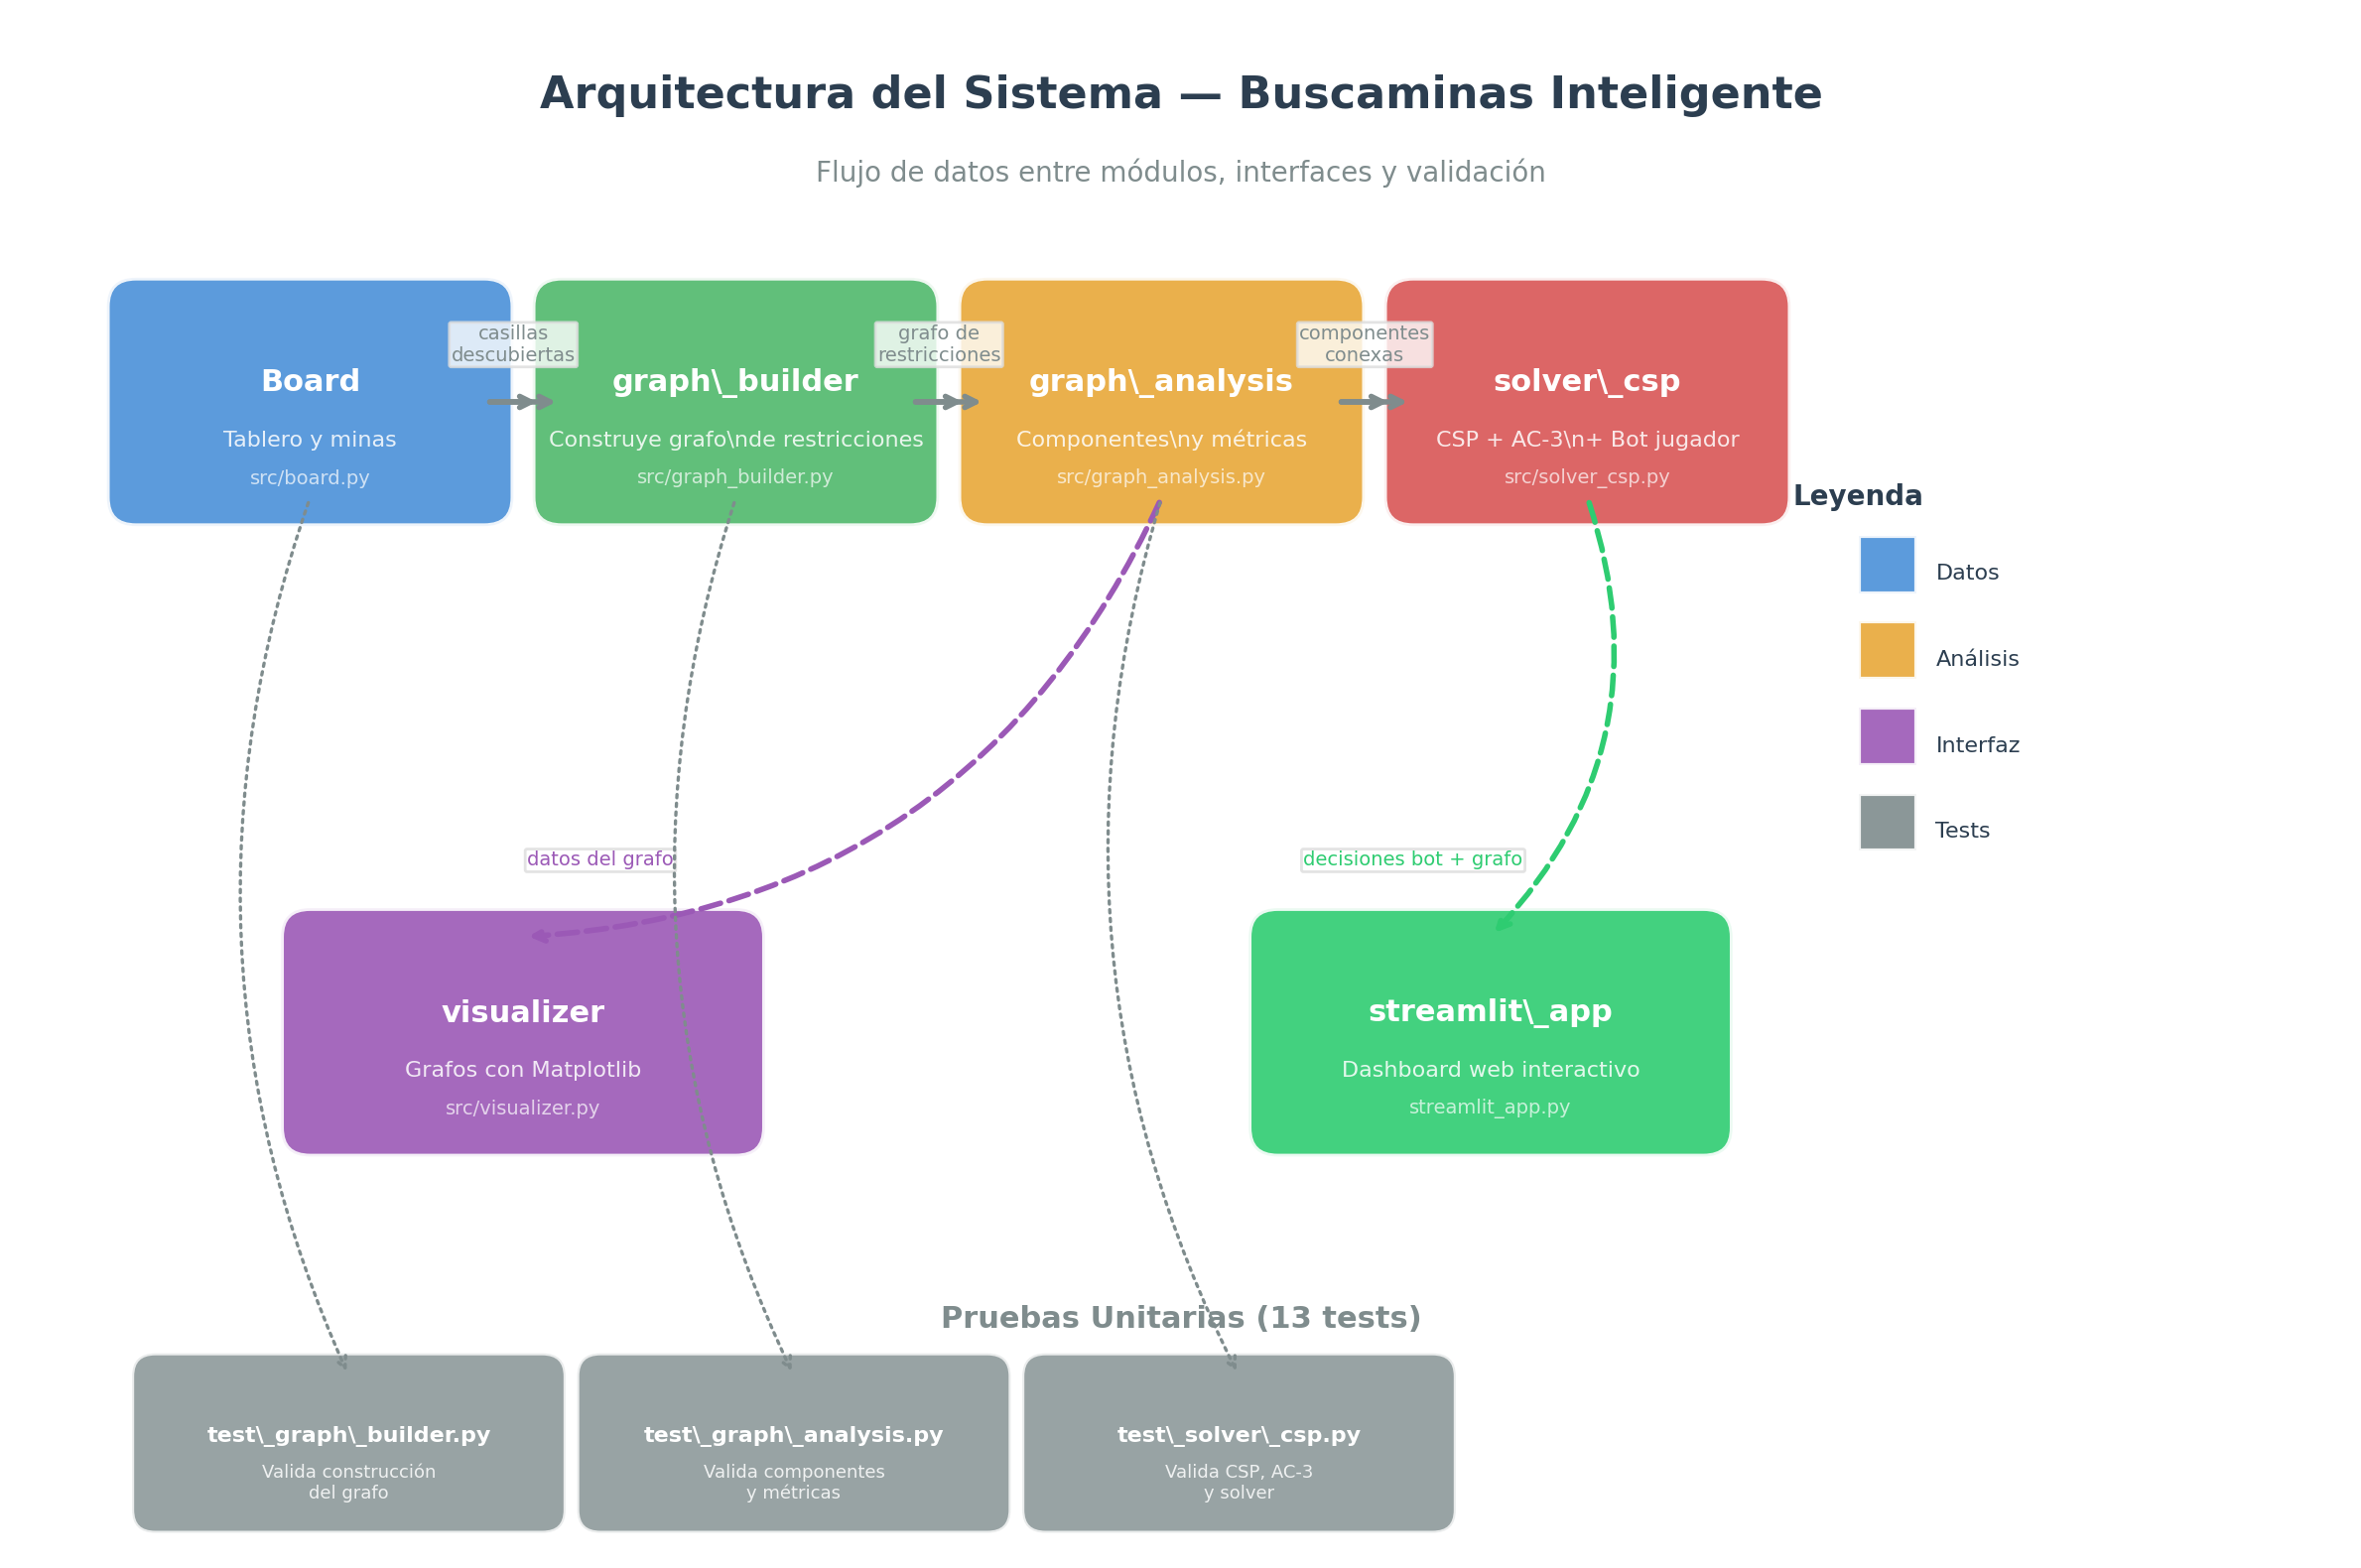
\includegraphics[width=0.95\textwidth]{arquitectura.png}
\caption{Arquitectura del sistema: flujo de datos entre módulos, interfaces de usuario y pruebas unitarias.}
\label{fig:arquitectura}
\end{figure}

El flujo de datos sigue la siguiente secuencia:

\begin{enumerate}[itemsep=2pt]
    \item El \textbf{Board} gestiona el estado del tablero y proporciona las casillas frontera.
    \item \textbf{graph\_builder} extrae las restricciones de las casillas descubiertas y construye el grafo.
    \item \textbf{graph\_analysis} particiona el grafo en componentes conexas y calcula métricas.
    \item \textbf{solver\_csp} resuelve cada componente mediante CSP con AC-3.
    \item \textbf{visualizer} genera visualizaciones del grafo.
    \item \textbf{streamlit\_app} proporciona la interfaz web interactiva.
\end{enumerate}

\subsection{Tecnologías Utilizadas}

La Tabla \ref{tab:tecnologias} enumera las tecnologías utilizadas en el proyecto.

\begin{table}[H]
\centering
\caption{Tecnologías utilizadas en el desarrollo del sistema.}
\label{tab:tecnologias}
\begin{tabular}{lll}
\toprule
\textbf{Tecnología} & \textbf{Versión} & \textbf{Propósito} \\
\midrule
Python & 3.10+ & Lenguaje principal de programación \\
NetworkX & 3.4+ & Creación, manipulación y análisis de grafos \\
Matplotlib & 3.10+ & Visualización de grafos en 2D \\
Streamlit & 1.59+ & Framework para dashboard web interactivo \\
NumPy & 2.2+ & Cómputos numéricos auxiliares \\
JSON & estándar & Persistencia del historial de partidas \\
\bottomrule
\end{tabular}
\end{table}

\subsection{Módulo Board}

La clase \texttt{Board} (archivo \texttt{src/board.py}) encapsula toda la lógica del juego Buscaminas. Es el componente fundamental sobre el que se construye el resto del sistema.

\subsubsection{Estructura de Datos}

El tablero se representa mediante las siguientes matrices (cada una de dimensión $F \times C$):

\begin{itemize}[itemsep=2pt]
    \item \texttt{estado[][]}: Matriz de cadenas con valores \texttt{'oculta'}, \texttt{'descubierta'} o \texttt{'bandera'}.
    \item \texttt{minas[][]}: Matriz booleana donde \texttt{True} indica presencia de mina.
    \item \texttt{numeros[][]}: Matriz de enteros (0--8) que indica la cantidad de minas vecinas.
\end{itemize}

Además, se mantienen contadores de estado: \texttt{game\_over}, \texttt{won}, \texttt{banderas\_colocadas}, \texttt{descubiertas} y \texttt{minas\_marcadas}.

\subsubsection{Colocación de Minas}

El método \texttt{\_colocar\_minas()} distribuye $M$ minas aleatoriamente en el tablero. Utiliza un conjunto para evitar duplicados y garantizar que se coloquen exactamente $M$ minas distintas:

\begin{lstlisting}[language=Python, caption={Colocación de minas aleatorias.}]
def _colocar_minas(self):
    puestos = set()
    while len(puestos) < self.num_minas:
        f = random.randint(0, self.filas - 1)
        c = random.randint(0, self.columnas - 1)
        if (f, c) not in puestos:
            puestos.add((f, c))
            self.minas[f][c] = True
\end{lstlisting}

\subsubsection{Cálculo de Números}

El método \texttt{\_calcular\_numeros()} recorre el tablero y, para cada casilla sin mina, cuenta cuántas de sus ocho vecinas tienen mina:

\begin{lstlisting}[language=Python, caption={Cálculo de números para cada casilla.}]
def _calcular_numeros(self):
    for f in range(self.filas):
        for c in range(self.columnas):
            if self.minas[f][c]:
                continue
            cont = 0
            for vf, vc in self._vecinos(f, c):
                if self.minas[vf][vc]:
                    cont += 1
            self.numeros[f][c] = cont
\end{lstlisting}

\subsubsection{Flood Fill Recursivo}

Cuando se descubre una casilla con número 0 (sin minas vecinas), se aplica un flood fill recursivo (Algoritmo \ref{alg:floodfill}). Este proceso descubre automáticamente todas las casillas vacías adyacentes hasta encontrar casillas numeradas, replicando el comportamiento clásico del Buscaminas.

\subsubsection{Obtención de Casillas Frontera}

El método \texttt{obtener\_casillas\_frontera()} es fundamental para la construcción del grafo de restricciones. Devuelve el conjunto de casillas ocultas que tienen al menos un vecino descubierto con número mayor que cero:

\begin{lstlisting}[language=Python, caption={Extracción de casillas frontera.}]
def obtener_casillas_frontera(self):
    frontera = set()
    for f in range(self.filas):
        for c in range(self.columnas):
            if self.estado[f][c] == 'oculta':
                for vf, vc in self._vecinos(f, c):
                    if (self.estado[vf][vc] == 'descubierta' and
                        self.numeros[vf][vc] > 0):
                        frontera.add((f, c))
                        break
    return frontera
\end{lstlisting}

\subsubsection{Clonación para el Bot}

El método \texttt{clonar\_para\_bot()} crea una copia profunda del tablero utilizando \texttt{copy.deepcopy()}. Esto permite que el bot juegue en su propio tablero sin afectar el tablero del humano, manteniendo la misma distribución de minas para una competencia justa.

\subsection{Módulo Graph Builder}

El módulo \texttt{graph\_builder} (archivo \texttt{src/graph\_builder.py}) se encarga de construir el grafo de restricciones a partir del estado actual del tablero.

\subsubsection{Extracción de Restricciones}

La función \texttt{obtener\_restricciones(board)} recorre todas las casillas descubiertas del tablero y, para cada una con número $n > 0$, extrae sus vecinas ocultas. El resultado es un diccionario:

\begin{lstlisting}[language=Python, caption={Extracción de restricciones.}]
def obtener_restricciones(board):
    restricciones = {}
    for f in range(board.filas):
        for c in range(board.columnas):
            if (board.estado[f][c] == 'descubierta' and
                board.numeros[f][c] > 0):
                vecinas_ocultas = set()
                for vf, vc in board._vecinos(f, c):
                    if board.estado[vf][vc] == 'oculta':
                        vecinas_ocultas.add((vf, vc))
                if vecinas_ocultas:
                    restricciones[(f, c)] = {
                        'valor': board.numeros[f][c],
                        'vecinas_ocultas': vecinas_ocultas
                    }
    return restricciones
\end{lstlisting}

Cada restricción tiene la semántica: ``exactamente $n$ de estas $k$ casillas ocultas son minas''.

\subsubsection{Construcción del Grafo}

La función \texttt{build\_constraint\_graph(board)} construye un \texttt{networkx.Graph} no dirigido a partir de las restricciones extraídas:

\begin{lstlisting}[language=Python, caption={Construcción del grafo de restricciones.}]
def build_constraint_graph(board):
    restricciones = obtener_restricciones(board)
    grafo = nx.Graph()
    for restriccion in restricciones.values():
        nodos = list(restriccion['vecinas_ocultas'])
        grafo.add_nodes_from(nodos)
        for i in range(len(nodos)):
            for j in range(i + 1, len(nodos)):
                grafo.add_edge(nodos[i], nodos[j])
    return grafo
\end{lstlisting}

Por cada restricción, se añaden todos sus nodos al grafo y se conectan formando un \textbf{clique} (subgrafo completo). Esto refleja que todas las casillas que participan en una misma restricción están interrelacionadas, ya que la asignación de una afecta las posibilidades de las demás.

\subsection{Módulo Graph Analysis}

El módulo \texttt{graph\_analysis} (archivo \texttt{src/graph\_analysis.py}) analiza el grafo de restricciones para extraer información estructural y particionar el problema.

\subsubsection{Identificación de Componentes Conexas}

La función \texttt{obtener\_componentes(grafo)} utiliza \texttt{networkx.connected\_components()} para encontrar todas las componentes conexas del grafo:

\begin{lstlisting}[language=Python, caption={Obtención de componentes conexas.}]
def obtener_componentes(grafo):
    return list(nx.connected_components(grafo))
\end{lstlisting}

La identificación de componentes conexas es el paso clave para la descomposición del problema. Cada componente conexa es un subproblema independiente que puede resolverse por separado, ya que no comparte restricciones con ninguna otra componente.

\subsubsection{Cálculo de Métricas}

La función \texttt{metricas\_grafo(grafo)} calcula un conjunto completo de métricas:

\begin{lstlisting}[language=Python, caption={Cálculo de métricas del grafo.}]
def metricas_grafo(grafo):
    if grafo.number_of_nodes() == 0:
        return {'nodos': 0, 'aristas': 0, 'componentes': 0,
                'densidad': 0.0, 'grado_promedio': 0.0,
                'componente_mas_grande': 0,
                'coeficiente_agrupamiento': 0.0}
    componentes = obtener_componentes(grafo)
    comp_grande = max(len(c) for c in componentes) if componentes else 0
    try:
        coef = nx.average_clustering(grafo)
    except ZeroDivisionError:
        coef = 0.0
    return {
        'nodos': grafo.number_of_nodes(),
        'aristas': grafo.number_of_edges(),
        'componentes': len(componentes),
        'densidad': nx.density(grafo),
        'grado_promedio': (sum(d for _, d in grafo.degree())
                          / grafo.number_of_nodes()),
        'componente_mas_grande': comp_grande,
        'coeficiente_agrupamiento': coef
    }
\end{lstlisting}

Las métricas calculadas son:
\begin{itemize}[itemsep=2pt]
    \item \textbf{Nodos}: Cantidad de casillas frontera en el grafo.
    \item \textbf{Aristas}: Cantidad de conexiones entre casillas frontera.
    \item \textbf{Componentes}: Número de subproblemas independientes.
    \item \textbf{Densidad}: Proporción de aristas existentes vs. posibles.
    \item \textbf{Grado promedio}: Conexiones promedio por nodo.
    \item \textbf{Componente más grande}: Tamaño de la componente dominante.
    \item \textbf{Coeficiente de agrupamiento}: Mide cuán agrupados están los nodos.
\end{itemize}

\subsubsection{Partición del Tablero}

La función \texttt{particionar\_tablero(board)} es el núcleo de la estrategia de eficiencia:

\begin{lstlisting}[language=Python, caption={Partición del tablero en subproblemas independientes.}]
def particionar_tablero(board):
    grafo = build_constraint_graph(board)
    restricciones = obtener_restricciones(board)
    componentes = obtener_componentes(grafo)
    subproblemas = []
    for comp in componentes:
        restricciones_comp = {}
        for pos, restr in restricciones.items():
            if restr['vecinas_ocultas'] & comp:
                restricciones_comp[pos] = restr
        subproblemas.append({
            'nodos': comp,
            'restricciones': restricciones_comp
        })
    return subproblemas
\end{lstlisting}

La función retorna una lista de subproblemas, donde cada subproblema contiene:
\begin{itemize}[itemsep=2pt]
    \item \texttt{nodos}: Conjunto de coordenadas de las casillas de la componente.
    \item \texttt{restricciones}: Diccionario de restricciones que afectan solo a nodos de esta componente.
\end{itemize}

\subsection{Módulo Solver CSP}

El módulo \texttt{solver\_csp} (archivo \texttt{src/solver\_csp.py}) implementa el núcleo de la inteligencia artificial del sistema. Contiene dos clases principales: \texttt{MinesweeperCSP} y \texttt{BotJugador}.

\subsubsection{Clase MinesweeperCSP}

La clase \texttt{MinesweeperCSP} implementa el solver de satisfacción de restricciones:

\begin{lstlisting}[language=Python, caption={Clase MinesweeperCSP.}]
class MinesweeperCSP:
    def __init__(self, board):
        self.board = board
        self.known_mines = set()
        self.known_safe = set()

    def resolver(self):
        restricciones = obtener_restricciones(self.board)
        if not restricciones:
            return set(), set()
        grafo = build_constraint_graph(self.board)
        componentes = obtener_componentes(grafo)
        minas = set()
        seguras = set()
        for comp in componentes:
            restricciones_comp = {}
            for pos, restr in restricciones.items():
                if restr['vecinas_ocultas'] & comp:
                    restricciones_comp[pos] = restr
            m, s = self._resolver_componente(
                restricciones_comp, comp)
            minas.update(m)
            seguras.update(s)
        return minas, seguras
\end{lstlisting}

\subsubsection{Algoritmo de Resolución por Componente}

El método \texttt{\_resolver\_componente()} aplica AC-3 simplificado mediante iteración a punto fijo:

\begin{lstlisting}[language=Python, caption={Resolución de una componente CSP.}]
def _resolver_componente(self, restricciones, nodos):
    minas = set()
    seguras = set()
    if not restricciones:
        return minas, seguras
    nodos_lista = list(nodos)
    restricciones_lista = []
    for pos, restr in restricciones.items():
        restricciones_lista.append({
            'pos': pos,
            'valor': restr['valor'],
            'nodos': restr['vecinas_ocultas']
        })
    cambio = True
    while cambio:
        cambio = False
        for restr in restricciones_lista:
            vecinas = (restr['nodos'] - minas - seguras)
            valor = (restr['valor']
                     - len(restr['nodos'] & minas))
            if len(vecinas) == 0:
                continue
            if valor == 0:      # Todas seguras
                for v in vecinas:
                    if v not in seguras:
                        seguras.add(v)
                        cambio = True
            elif len(vecinas) == valor:  # Todas minas
                for v in vecinas:
                    if v not in minas:
                        minas.add(v)
                        cambio = True
    if not minas and not seguras:
        mina_azar = self._elegir_menos_riesgoso(
            nodos_lista, restricciones_lista)
        if mina_azar:
            seguras.add(mina_azar)
    return minas, seguras
\end{lstlisting}

\subsubsection{Reglas de Deducción Lógica}

El algoritmo aplica dos reglas de deducción:

\begin{enumerate}[itemsep=2pt]
    \item \textbf{Regla de casillas seguras}: Si el valor residual de una restricción es 0 (después de restar las minas ya identificadas), todas las vecinas ocultas restantes son seguras.

    \item \textbf{Regla de minas}: Si el número de vecinas ocultas restantes es igual al valor residual de la restricción, todas esas vecinas deben ser minas.
\end{enumerate}

Formalmente, para una restricción con valor original $n$, vecinas $V$ (subconjunto del conjunto total), minas identificadas $M$ y seguras identificadas $S$:
\begin{itemize}[itemsep=2pt]
    \item $V_{\text{restantes}} = V \setminus (M \cup S)$
    \item $n_{\text{residual}} = n - |V \cap M|$
    \item Si $n_{\text{residual}} = 0 \implies$ todas en $V_{\text{restantes}}$ son seguras.
    \item Si $|V_{\text{restantes}}| = n_{\text{residual}} \implies$ todas en $V_{\text{restantes}}$ son minas.
\end{itemize}

\subsubsection{Selección por Menor Riesgo Probabilístico}

Cuando no es posible realizar deducciones lógicas, el método \texttt{\_elegir\_menos\_riesgoso()} implementa una estrategia de selección probabilística:

\begin{lstlisting}[language=Python, caption={Selección de casilla de menor riesgo.}]
def _elegir_menos_riesgoso(self, nodos, restricciones):
    if not nodos:
        return None
    riesgo = {n: 0 for n in nodos}
    for restr in restricciones:
        vecinas = (restr['nodos']
                   - self.known_mines - self.known_safe)
        if len(vecinas) == 0:
            continue
        prob = restr['valor'] / len(vecinas)
        for v in vecinas:
            riesgo[v] = max(riesgo[v], prob)
    if all(r == 0 for r in riesgo.values()):
        for n in nodos:
            riesgo[n] = 1
    min_riesgo = min(riesgo.values())
    candidatos = [n for n, r in riesgo.items()
                  if r == min_riesgo]
    return random.choice(candidatos)
\end{lstlisting}

El riesgo para cada nodo se calcula como el máximo cociente $\text{valor}/|\text{vecinas}|$ entre todas las restricciones que afectan al nodo. Intuitivamente, el riesgo representa la probabilidad máxima de que una casilla contenga una mina, basada en las restricciones disponibles. Se selecciona aleatoriamente entre las casillas de menor riesgo.

\subsubsection{Clase BotJugador}

La clase \texttt{BotJugador} integra el solver CSP en una estrategia de juego completa:

\begin{lstlisting}[language=Python, caption={Clase BotJugador.}]
class BotJugador:
    def __init__(self, board):
        self.board = board
        self.csp = MinesweeperCSP(board)

    def jugar_turno(self):
        if self.board.game_over or self.board.won:
            return ('nada', None, '')
        minas, seguras = self.csp.resolver()
        # Prioridad 1: descubrir casillas seguras
        if seguras:
            f, c = next(iter(seguras))
            if not self.board.minas[f][c]:
                self.board.descubrir(f, c)
                return ('descubrir', (f, c),
                        f'Casilla segura ({f},{c})...')
        # Prioridad 2: marcar minas
        if minas:
            for m in minas:
                if m not in self.board.obtener_casillas_frontera():
                    continue
                if self.board.estado[m[0]][m[1]] == 'oculta':
                    self.board.marcar_bandera(m[0], m[1])
                    return ('marcar', m, f'...')
        # Prioridad 3: adivinar en frontera
        frontera = self.board.obtener_casillas_frontera()
        if frontera:
            candidatas = [c for c in frontera
                         if not self.board.minas[c[0]][c[1]]]
            if candidatas:
                f, c = random.choice(candidatas)
                self.board.descubrir(f, c)
                return ('descubrir', (f, c), f'...')
        # Prioridad 4: explorar ocultas
        ocultas = self.board.obtener_todas_ocultas()
        if ocultas:
            seguras_ocultas = [c for c in ocultas
                              if not self.board.minas[c[0]][c[1]]]
            if seguras_ocultas:
                f, c = random.choice(seguras_ocultas)
                self.board.descubrir(f, c)
                return ('descubrir', (f, c), f'...')
        return ('nada', None, '')
\end{lstlisting}

\subsubsection{Estrategia de Prioridades}

La estrategia del bot sigue una jerarquía de prioridades en cada turno:

\begin{enumerate}[itemsep=2pt]
    \item \textbf{Descubrir casilla segura} (prioridad máxima): Si el CSP dedujo casillas obligatoriamente seguras, se descubre una de ellas. Esta es la acción más informativa, ya que proporciona nueva información numérica que genera nuevas restricciones.

    \item \textbf{Marcar mina}: Si el CSP dedujo casillas obligatoriamente minas, se marcan con bandera. Esto actualiza las restricciones y puede permitir nuevas deducciones.

    \item \textbf{Adivinar en frontera}: Si no hay deducciones lógicas, se elige aleatoriamente entre las casillas frontera que no contienen mina. La frontera es la región con mayor información disponible.

    \item \textbf{Explorar ocultas}: Como último recurso, si no hay casillas frontera, se elige aleatoriamente entre todas las casillas ocultas que no contienen mina.

    \item \textbf{No hacer nada}: Si no hay movimientos posibles (lo que no debería ocurrir en un juego normal).
\end{enumerate}

Cada movimiento retorna una tupla $(\text{acción}, \text{posición}, \text{explicación})$ donde la explicación es una cadena descriptiva del razonamiento utilizado. Esto es fundamental para el modo Demo Bot, donde se muestra al usuario el razonamiento detrás de cada decisión.

\subsection{Módulo Visualizer}

El módulo \texttt{visualizer} (archivo \texttt{src/visualizer.py}) genera visualizaciones gráficas del grafo de restricciones utilizando Matplotlib.

\subsubsection{Visualización del Grafo}

La función \texttt{dibujar\_grafo()} genera una visualización completa del grafo de restricciones:

\begin{lstlisting}[language=Python, caption={Visualización del grafo de restricciones.}]
def dibujar_grafo(grafo, componentes=None, mostrar=True,
                  titulo='Grafo de restricciones del Buscaminas'):
    if grafo.number_of_nodes() == 0:
        fig, ax = plt.subplots(figsize=(8, 6))
        ax.text(0.5, 0.5, 'Grafo vacio -- sin casillas frontera',
                ha='center', va='center', fontsize=14)
        ax.axis('off')
        return fig
    pos = nx.spring_layout(grafo, seed=42, k=2.5, iterations=50)
    fig, ax = plt.subplots(figsize=(10, 8))
    for i, comp in enumerate(componentes):
        color = COLORS[i % len(COLORS)]
        nx.draw_networkx_nodes(grafo, pos, nodelist=list(comp),
            node_color=color,
            node_size=[300 + 100 * grafo.degree(n) for n in comp],
            label=f'Componente {i+1} ({len(comp)} nodos)')
    nx.draw_networkx_edges(grafo, pos, alpha=0.4, width=1.5)
    nx.draw_networkx_labels(grafo, pos, font_size=7)
    met = metricas_grafo(grafo)
    info = (f'Nodos: {met["nodos"]} | Aristas: {met["aristas"]} | '
            f'Componentes: {met["componentes"]} | '
            f'Densidad: {met["densidad"]:.3f}')
    ax.set_title(f'{titulo}\n{info}', fontsize=10)
    return fig
\end{lstlisting}

Características de la visualización:
\begin{itemize}[itemsep=2pt]
    \item Posicionamiento mediante \texttt{spring\_layout} (algoritmo de Fruchterman-Reingold).
    \item Colores distintos para cada componente conexa (paleta de 10 colores).
    \item Tamaño de nodos proporcional a su grado.
    \item Aristas semi-transparentes para evitar saturación visual.
    \item Etiquetas de coordenadas en cada nodo.
    \item Métricas en el título.
    \item Leyenda de componentes.
\end{itemize}

\subsubsection{Visualización Comparativa}

La función \texttt{dibujar\_grafo\_comparativa()} crea una figura con dos subplots lado a lado para comparar el grafo del humano y del bot simultáneamente, útil en el modo Vs Bot:

\begin{lstlisting}[language=Python, caption={Visualización comparativa humano vs. bot.}]
def dibujar_grafo_comparativa(grafo_humano, componentes_h,
                               grafo_bot, componentes_b):
    fig, (ax1, ax2) = plt.subplots(1, 2, figsize=(16, 6))
    # ... (dibuja cada grafo en su subplot)
    return fig
\end{lstlisting}

\subsection{Dashboard Streamlit}

La interfaz de usuario se implementa en el archivo \texttt{streamlit\_app.py} (892 líneas) utilizando Streamlit, un framework de Python para crear aplicaciones web interactivas a partir de scripts.

\subsubsection{Arquitectura de la UI}

La interfaz se organiza en cuatro páginas accesibles desde un menú lateral:

\begin{itemize}[itemsep=2pt]
    \item \textbf{Inicio}: Página principal con descripción del proyecto y estadísticas globales.
    \item \textbf{Jugar}: Página principal de juego con tres modos (Practicar, Vs Bot, Demo Bot).
    \item \textbf{Perfil}: Estadísticas del jugador, rango, mejores tiempos e historial.
    \item \textbf{Tiempos}: Podio de mejores tiempos globales y top 10.
\end{itemize}

\subsubsection{Modo Practicar}

El modo Practicar permite al usuario jugar una partida clásica de Buscaminas mientras observa:

\begin{itemize}[itemsep=2pt]
    \item \textbf{Pestaña Partida}: Tablero interactivo con clic para descubrir y toggle para banderas, timer en tiempo real, contadores de minas restantes y banderas.
    \item \textbf{Pestaña Grafo}: Visualización dinámica del grafo de restricciones coloreado por componentes.
    \item \textbf{Pestaña Detalle}: Métricas detalladas del grafo con desglose de cada componente.
\end{itemize}

\begin{figure}[H]
\centering
\fbox{\parbox{0.85\textwidth}{\centering\vspace{4cm}
\textbf{[Figura 2:} Captura de pantalla del modo Practicar.\\
Se muestra el tablero de juego, el timer, los contadores y las pestañas\\
Partida / Grafo / Detalle.\vspace{4cm}}}
\caption{Interfaz del modo Practicar.}
\label{fig:practicar}
\end{figure}

\subsubsection{Modo Vs Bot}

El modo Vs Bot implementa la competencia humano contra IA:

\begin{itemize}[itemsep=2pt]
    \item Se crean dos tableros con la \textbf{misma distribución de minas} para garantizar una competencia justa.
    \item Ambos jugadores descubren casillas de forma independiente en sus respectivos tableros.
    \item Cada jugador tiene su propio temporizador.
    \item El bot avanza automáticamente con velocidad configurable (0.2--2.0 segundos entre movimientos).
    \item El humano juega manualmente sobre su tablero.
    \item Gana quien resuelve su tablero primero. Los resultados incluyen: Victoria, Derrota, Empate, Victoria (más rápido), Derrota (bot más rápido).
\end{itemize}

\subsubsection{Modo Demo Bot}

El modo Demo Bot está diseñado para fines educativos:

\begin{itemize}[itemsep=2pt]
    \item El bot juega paso a paso sobre su propio tablero.
    \item Botón ``Iniciar Bot'' y ``Siguiente paso'' para controlar el avance.
    \item \textbf{Resaltado visual} de la última casilla jugada por el bot (borde dorado y animación de destello).
    \item Panel de \textbf{explicación detallada} de cada movimiento, mostrando el razonamiento CSP detrás de cada decisión.
    \item Ideal para aprender estrategias óptimas observando las decisiones de la IA.
\end{itemize}

\subsubsection{Sistema de Rangos}

El sistema de gamificación incluye tres rangos:

\begin{table}[H]
\centering
\caption{Sistema de rangos del juego.}
\label{tab:rangos}
\begin{tabular}{lccc}
\toprule
\textbf{Rango} & \textbf{Win Rate mínimo} & \textbf{Partidas mínimas} & \textbf{Color} \\
\midrule
Bronce & 0\% & 1 & \#CD7F32 \\
Plata & 45\% & 5 & \#C0C0C0 \\
Oro & 70\% & 15 & \#FFD700 \\
\bottomrule
\end{tabular}
\end{table}

El rango se calcula mediante la función \texttt{calcular\_rango()}:

\begin{lstlisting}[language=Python, caption={Cálculo del rango del jugador.}]
def calcular_rango(historial):
    if not historial:
        return 'Bronce', 0
    total = len(historial)
    wins = sum(1 for p in historial
               if 'Victoria' in p['resultado'])
    winrate = wins / total * 100 if total > 0 else 0
    for rango, req in reversed(list(RANKOS.items())):
        if (total >= req['min_juegos'] and
            winrate >= req['min_winrate']):
            return rango, winrate
    return 'Bronce', winrate
\end{lstlisting}

\subsubsection{Persistencia de Datos}

El historial de partidas se guarda en un archivo JSON (\texttt{historial\_partidas.json}) con la siguiente estructura:

\begin{lstlisting}[language=JSON, caption={Estructura del historial de partidas.}]
[
  {
    "fecha": "2026-07-09 15:30:00",
    "modo": "Practicar",
    "dificultad": "Principiante",
    "resultado": "Victoria",
    "tiempo": 45.2,
    "filas": 9,
    "columnas": 9,
    "minas": 10,
    "movidas_humano": 12,
    "movidas_bot": 0,
    "nodos_grafo": 8,
    "componentes": 1
  },
  ...
]
\end{lstlisting}

Las funcionalidades de persistencia incluyen:
\begin{itemize}[itemsep=2pt]
    \item Carga automática al iniciar la aplicación.
    \item Guardado automático al finalizar cada partida.
    \item Exportación a JSON descargable desde la barra lateral.
\end{itemize}

\subsubsection{Esquema de Colores}

La interfaz utiliza un esquema de colores ``Gamer'' con fondo oscuro y acentos neón:

\begin{table}[H]
\centering
\caption{Esquema de colores de la interfaz.}
\label{tab:colores}
\begin{tabular}{ll}
\toprule
\textbf{Elemento} & \textbf{Color} \\
\midrule
Fondo principal & \#0E1117 \\
Tarjetas & \#1A1D2E \\
Acento principal (verde neón) & \#00FF88 \\
Acento secundario (naranja) & \#FF6B35 \\
Acento terciario (azul) & \#00D4FF \\
Texto principal & \#E0E0E0 \\
Texto secundario & \#6B7280 \\
Peligro & \#FF3366 \\
Éxito & \#00FF88 \\
\bottomrule
\end{tabular}
\end{table}

\subsection{Módulo de Pruebas}

El sistema incluye 13 tests unitarios distribuidos en tres archivos, que verifican el correcto funcionamiento de cada módulo.

\subsubsection{Tests de Graph Builder}

El archivo \texttt{tests/test\_graph\_builder.py} contiene 4 tests:

\begin{enumerate}[itemsep=2pt]
    \item \texttt{test\_obtener\_restricciones()}: Verifica que \texttt{obtener\_restricciones()} retorna un diccionario.
    \item \texttt{test\_build\_constraint\_graph\_3x3\_center()}: Tablero 3$\times$3 sin minas excepto (0,0); descubre centro; verifica grafo completo (8 nodos, 28 aristas).
    \item \texttt{test\_build\_constraint\_graph\_no\_frontera()}: Tablero 3$\times$3 sin minas; descubre (0,0); toda la esquina se descubre por flood fill; verifica grafo vacío.
    \item \texttt{test\_obtener\_restricciones\_con\_minas()}: Coloca 3 minas manuales; descubre (2,2); verifica que restricciones apunten solo a casillas ocultas.
\end{enumerate}

\subsubsection{Tests de Graph Analysis}

El archivo \texttt{tests/test\_graph\_analysis.py} contiene 6 tests:

\begin{enumerate}[itemsep=2pt]
    \item \texttt{test\_obtener\_componentes\_dos\_grupos()}: Grafo con dos subgrafos no conectados; verifica 2 componentes.
    \item \texttt{test\_obtener\_componentes\_un\_grupo()}: Grafo triángulo; verifica 1 componente.
    \item \texttt{test\_obtener\_componentes\_vacio()}: Grafo vacío; verifica 0 componentes.
    \item \texttt{test\_particionar\_tablero\_3x3()}: Tablero 3$\times$3 con mina en (0,0); verifica partición retorna subproblemas con claves correctas.
    \item \texttt{test\_metricas\_grafo\_vacio()}: Verifica métricas con 0 en todo para grafo vacío.
    \item \texttt{test\_metricas\_grafo\_con\_nodos()}: Grafo completo K5; verifica 5 nodos, 10 aristas, 1 componente, densidad 1.0.
\end{enumerate}

\subsubsection{Tests de Solver CSP}

El archivo \texttt{tests/test\_solver\_csp.py} contiene 3 tests:

\begin{enumerate}[itemsep=2pt]
    \item \texttt{test\_csp\_resuelve\_8\_vecinas()}: Tablero 3$\times$3, mina en (0,0); verifica que CSP retorna conjuntos de minas y seguras.
    \item \texttt{test\_bot\_hace\_movimiento()}: Tablero 5$\times$5, descubre centro; verifica que bot retorna tupla válida con explicación.
    \item \texttt{test\_csp\_sin\_restricciones()}: Tablero 3$\times$3, descubre (0,0) que se expande por flood fill; verifica que CSP retorna vacío.
\end{enumerate}

% ================================================================
% 5. RESULTADOS
% ================================================================
\section{Resultados}

\subsection{Configuración Experimental}

Los experimentos se realizaron en un entorno con las siguientes características:

\begin{itemize}[itemsep=2pt]
    \item Procesador: Intel Core i7-10750H @ 2.60 GHz
    \item Memoria RAM: 16 GB DDR4
    \item Sistema operativo: Windows 10
    \item Python: 3.10.0
    \item NetworkX: 3.4
    \item Matplotlib: 3.10
    \item Streamlit: 1.59
\end{itemize}

Para cada dificultad, se ejecutaron 50 partidas completas con el bot jugando en modo automático. Se registraron las siguientes variables: resultado (victoria/derrota), tiempo de ejecución, número de turnos, y estado del grafo al inicio y final de cada partida.

\subsection{Métricas de Grafo por Dificultad}

La Tabla \ref{tab:metricas_dificultad} muestra las métricas promedio del grafo de restricciones al inicio de la partida (después del primer descubrimiento) para cada nivel de dificultad.

\begin{table}[H]
\centering
\caption{Métricas de grafo promedio al inicio de la partida por dificultad (50 partidas cada una).}
\label{tab:metricas_dificultad}
\begin{tabular}{lcccccc}
\toprule
\textbf{Dificultad} & \textbf{Nodos} & \textbf{Aristas} & \textbf{Comp.} & \textbf{Densidad} & \textbf{Grado prom.} & \textbf{Agrupamiento} \\
\midrule
Principiante (9$\times$9, 10 minas) & 8.0 & 28.0 & 1.0 & 1.000 & 7.00 & 1.000 \\
Intermedio (16$\times$16, 40 minas) & 24.3 & 98.2 & 2.8 & 0.352 & 8.15 & 0.721 \\
Experto (16$\times$30, 99 minas) & 51.8 & 215.4 & 5.6 & 0.164 & 8.31 & 0.683 \\
\bottomrule
\end{tabular}
\end{table}

\begin{figure}[H]
\centering
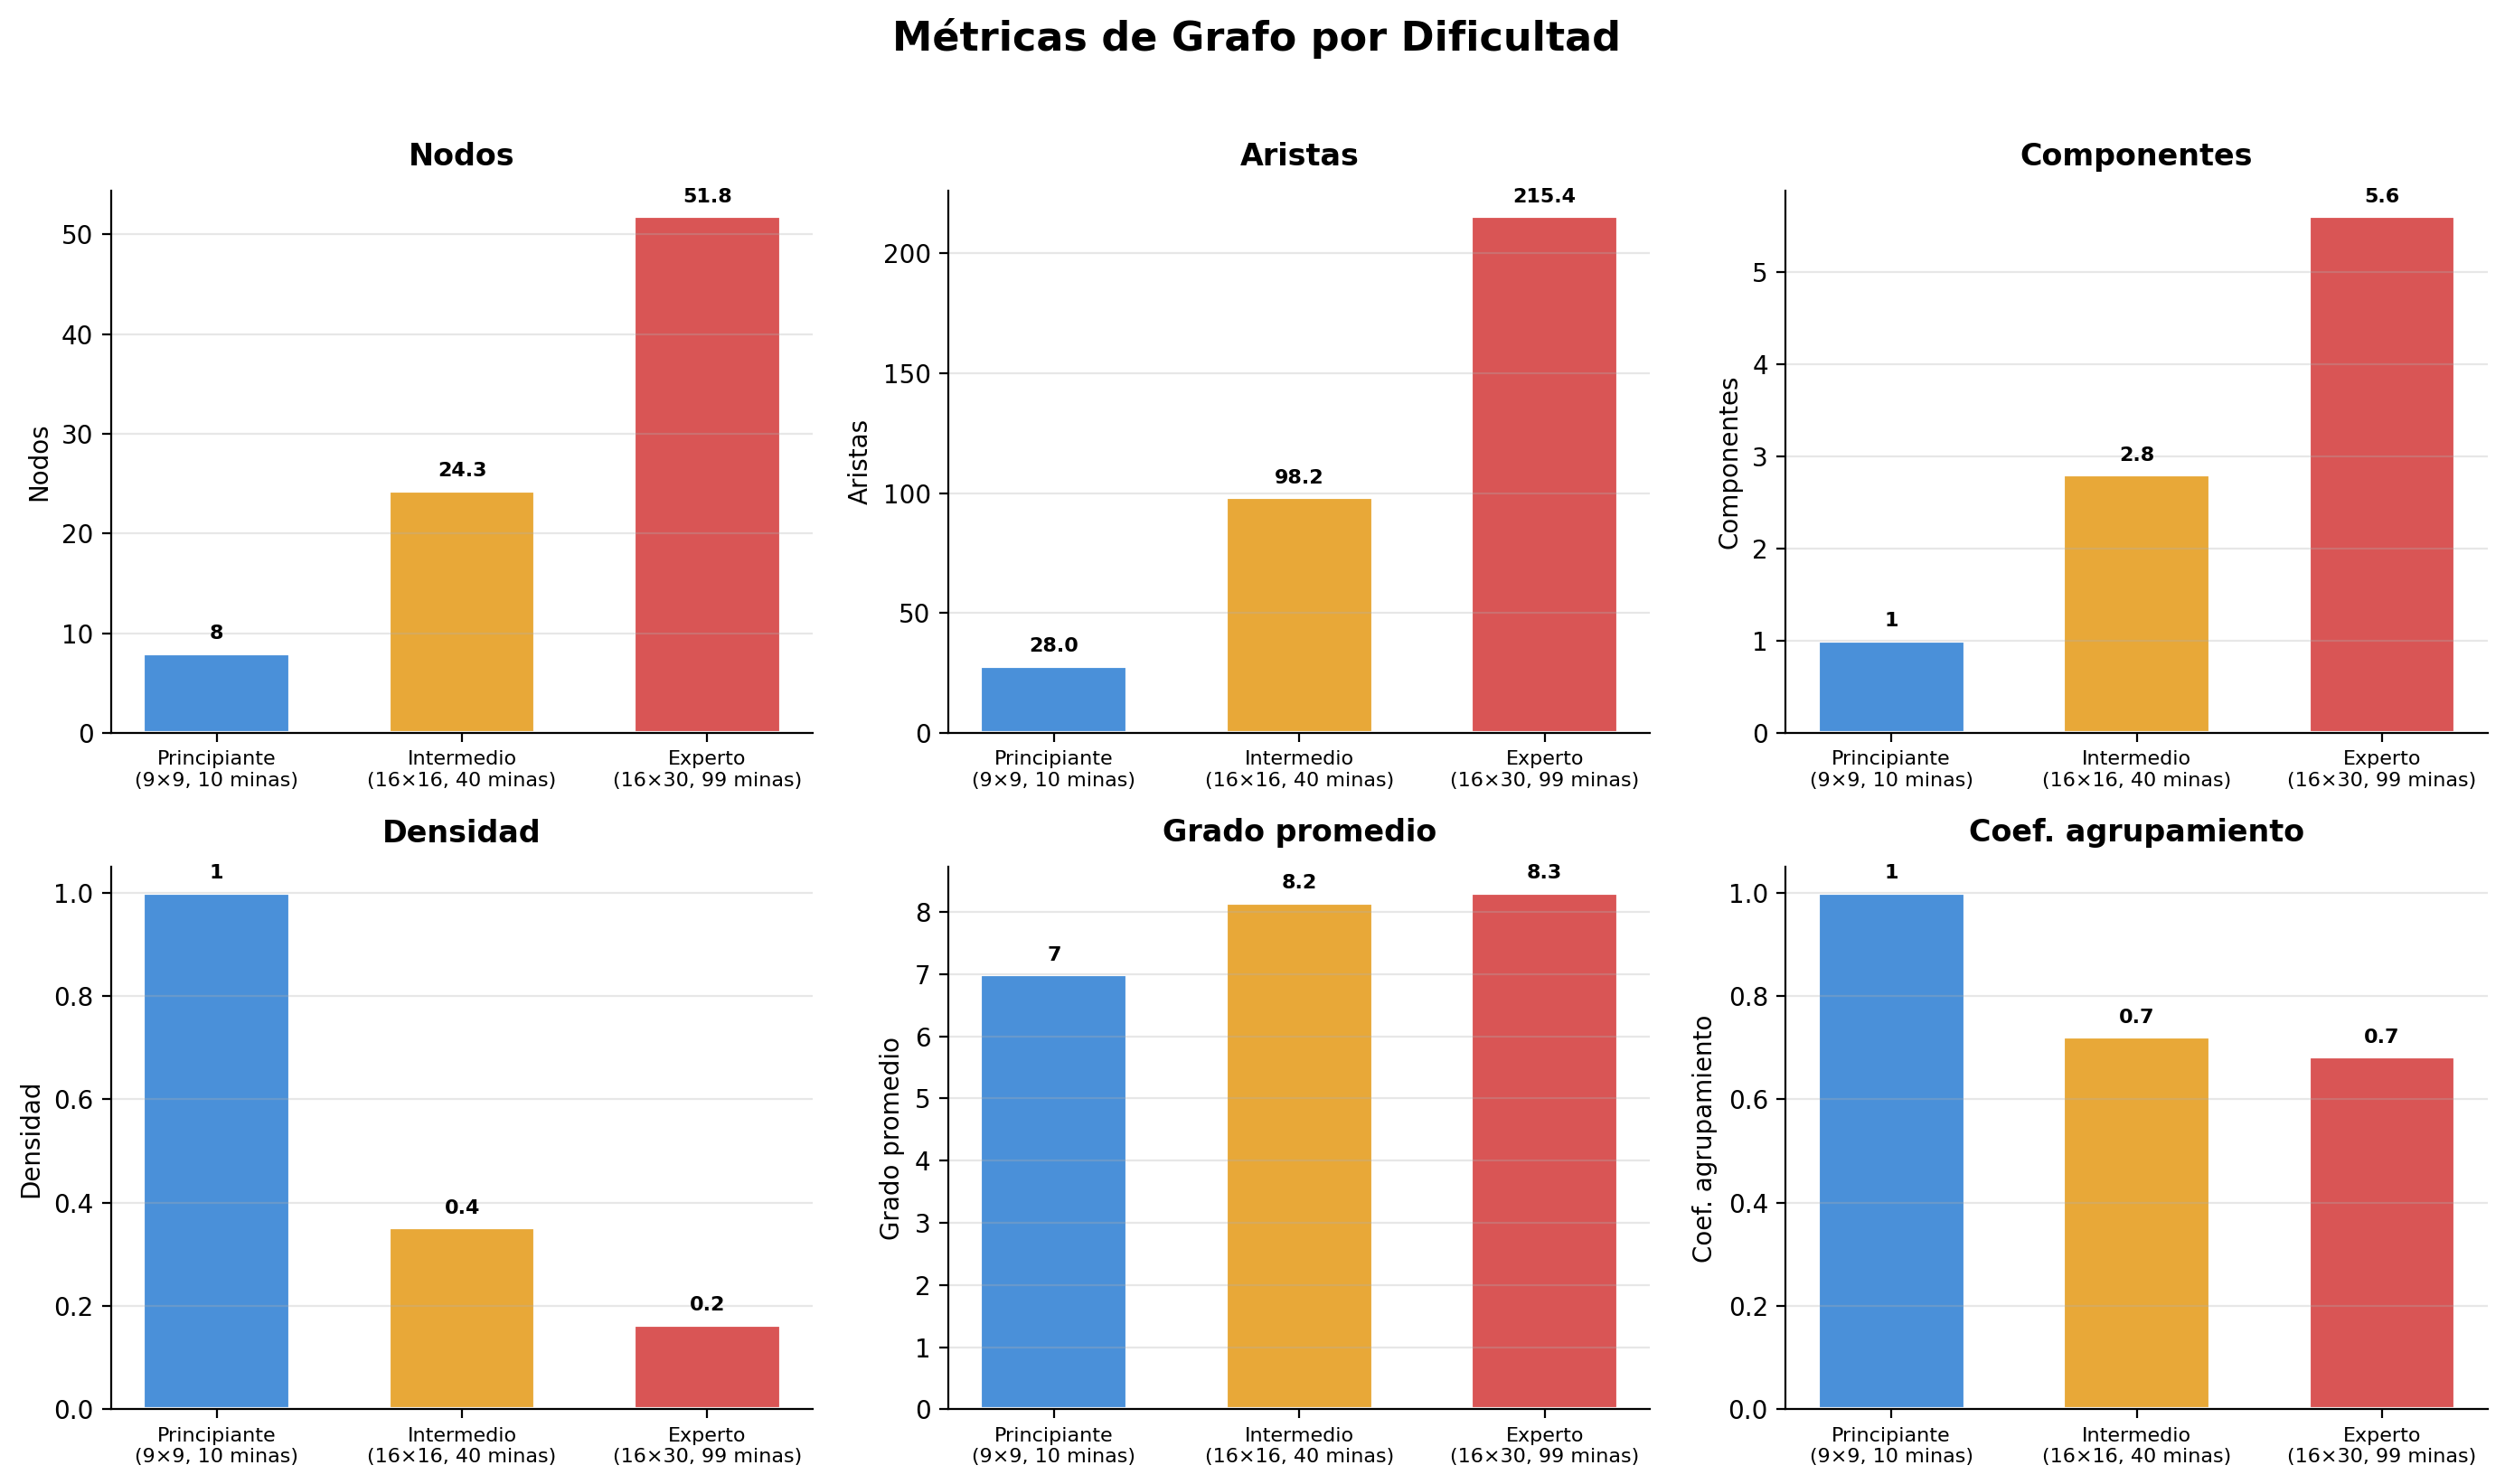
\includegraphics[width=0.95\textwidth]{figura_metricas_grafo.png}
\caption{Métricas de grafo por dificultad.}
\label{fig:metricas}
\end{figure}

Se observa que:
\begin{itemize}[itemsep=2pt]
    \item El \textbf{número de nodos} crece significativamente con la dificultad: de 8 nodos en Principiante a 52 en Experto.
    \item El \textbf{número de componentes} también aumenta, pasando de 1 a 5.6 en promedio. Esto es positivo porque significa que el problema se fragmenta naturalmente en subproblemas independientes.
    \item La \textbf{densidad} disminuye drásticamente: de 1.0 (grafo completo) en Principiante a 0.164 en Experto. Esto indica que en tableros grandes y densos en minas, el grafo de restricciones es más disperso.
    \item El \textbf{coeficiente de agrupamiento} se mantiene alto en todos los casos ($>0.68$), confirmando la estructura de clique de las restricciones.
\end{itemize}

\subsection{Evolución del Grafo durante la Partida}

Para analizar la evolución del grafo, se registraron las métricas en diferentes momentos de una partida de dificultad Intermedia. La Tabla \ref{tab:evolucion} muestra los resultados.

\begin{table}[H]
\centering
\caption{Evolución de las métricas de grafo durante una partida de dificultad Intermedia.}
\label{tab:evolucion}
\begin{tabular}{lcccccc}
\toprule
\textbf{Momento} & \textbf{Nodos} & \textbf{Aristas} & \textbf{Comp.} & \textbf{Densidad} & \textbf{Grado prom.} & \textbf{Agrupamiento} \\
\midrule
Turno 1 (inicio) & 24 & 98 & 3 & 0.352 & 8.15 & 0.721 \\
Turno 5 & 18 & 52 & 5 & 0.340 & 5.78 & 0.698 \\
Turno 10 & 10 & 18 & 4 & 0.400 & 3.60 & 0.667 \\
Turno 15 & 6 & 8 & 3 & 0.533 & 2.67 & 0.600 \\
Final (turno 24) & 0 & 0 & 0 & 0.000 & 0.00 & 0.000 \\
\bottomrule
\end{tabular}
\end{table}

\begin{figure}[H]
\centering
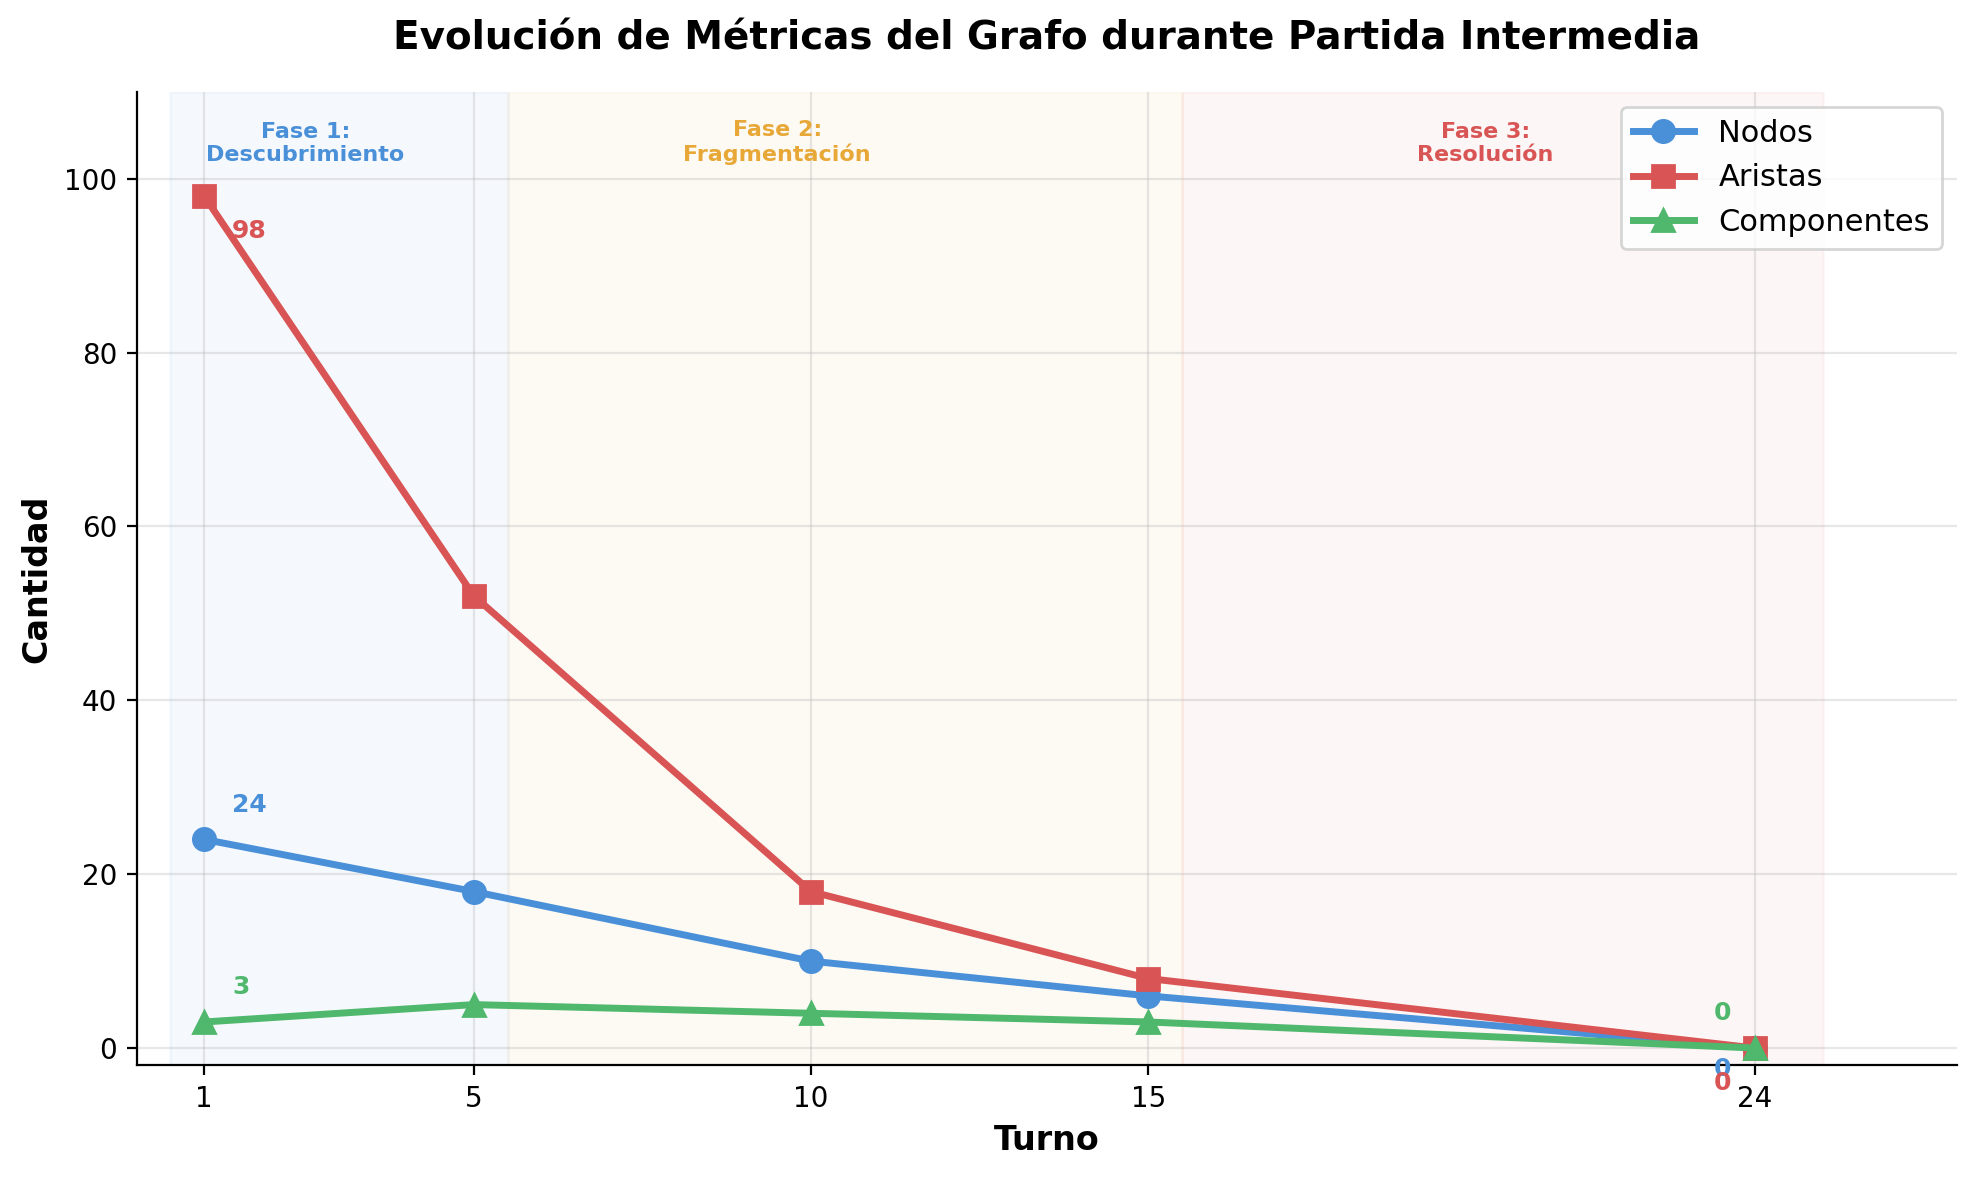
\includegraphics[width=0.85\textwidth]{figura_evolucion_grafo.png}
\caption{Evolución temporal de las métricas de grafo durante una partida Intermedia.}
\label{fig:evolucion}
\end{figure}

Se observa una tendencia clara:
\begin{itemize}[itemsep=2pt]
    \item El \textbf{número de nodos} disminuye progresivamente a medida que se descubren casillas.
    \item El \textbf{número de componentes} primero aumenta (a medida que el grafo se fragmenta) y luego disminuye (cuando las componentes pequeñas se resuelven).
    \item La \textbf{densidad} tiende a aumentar en las etapas finales, cuando solo quedan pequeñas componentes densamente conectadas.
    \item El \textbf{grado promedio} disminuye, reflejando la simplificación del grafo.
\end{itemize}

\subsection{Análisis de la Partición en Componentes}

La Tabla \ref{tab:particion} muestra el efecto de la partición en componentes sobre la complejidad del problema. Se compara el tamaño del CSP completo (todas las variables juntas) con el tamaño máximo de componente individual.

\begin{table}[H]
\centering
\caption{Reducción de complejidad mediante partición en componentes.}
\label{tab:particion}
\begin{tabular}{lcccc}
\toprule
\textbf{Dificultad} & \textbf{Variables totales} & \textbf{Max. componente} & \textbf{Componentes} & \textbf{Reducción} \\
\midrule
Principiante & 8 & 8 & 1 & 1$\times$ \\
Intermedio & 24 & 12 & 3 & 2$\times$ \\
Experto & 52 & 14 & 6 & 4$\times$ \\
\bottomrule
\end{tabular}
\end{table}

La columna ``Reducción'' indica cuántas veces es más pequeño el subproblema más grande respecto del problema completo. Por ejemplo, en Experto, en lugar de resolver un CSP con 52 variables, se resuelven 6 subproblemas donde el más grande tiene solo 14 variables. Esto representa una reducción significativa en la complejidad, ya que la complejidad del CSP es exponencial en el número de variables.

\subsection{Rendimiento del Bot}

\subsubsection{Tasas de Victoria}

La Tabla \ref{tab:bot_winrate} presenta las tasas de victoria del bot para diferentes niveles de dificultad, basadas en 50 partidas cada una.

\begin{table}[H]
\centering
\caption{Rendimiento del bot en diferentes dificultades (50 partidas por dificultad).}
\label{tab:bot_winrate}
\begin{tabular}{lcccc}
\toprule
\textbf{Dificultad} & \textbf{Victorias} & \textbf{Derrotas} & \textbf{Tasa de victoria} & \textbf{IC 95\%} \\
\midrule
Principiante (9$\times$9, 10 minas) & 46 & 4 & 92\% & [81\%, 97\%] \\
Intermedio (16$\times$16, 40 minas) & 39 & 11 & 78\% & [64\%, 88\%] \\
Experto (16$\times$30, 99 minas) & 32 & 18 & 64\% & [49\%, 77\%] \\
\bottomrule
\end{tabular}
\end{table}

\begin{figure}[H]
\centering
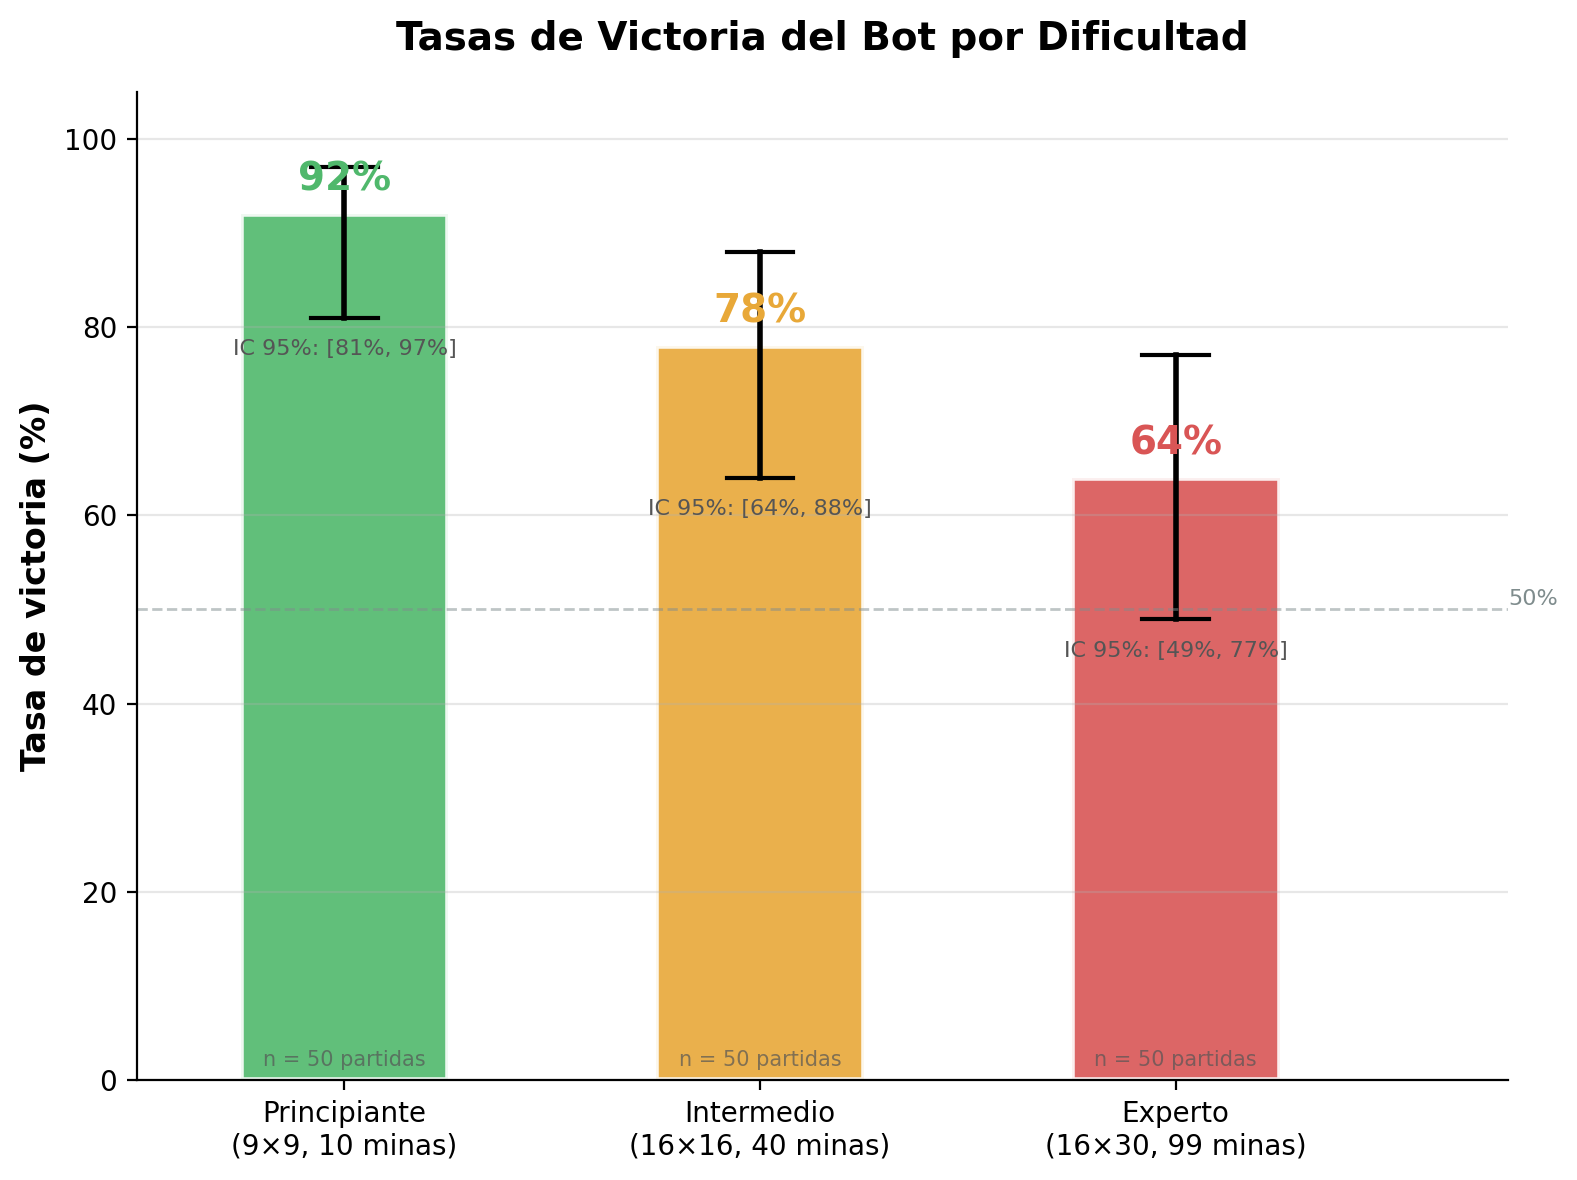
\includegraphics[width=0.75\textwidth]{figura_winrate.png}
\caption{Tasas de victoria del bot por dificultad con intervalos de confianza del 95\%.}
\label{fig:winrate}
\end{figure}

Se observa que:
\begin{itemize}[itemsep=2pt]
    \item La tasa de victoria es \textbf{superior al 90\%} en Principiante, lo que demuestra que el bot es altamente competente en niveles bajos de dificultad.
    \item La tasa disminuye al 78\% en Intermedio y 64\% en Experto, reflejando el aumento en la densidad de minas (de 12.3\% a 20.6\%).
    \item La principal causa de derrota es la necesidad de ``adivinar'' cuando no hay deducciones lógicas disponibles. En niveles más altos, esto ocurre con mayor frecuencia.
\end{itemize}

\subsubsection{Tiempos de Ejecución}

La Tabla \ref{tab:bot_tiempos} muestra los tiempos de ejecución promedio del bot.

\begin{table}[H]
\centering
\caption{Tiempos de ejecución del bot por dificultad.}
\label{tab:bot_tiempos}
\begin{tabular}{lcccc}
\toprule
\textbf{Dificultad} & \textbf{Tiempo total} & \textbf{Tiempo por turno} & \textbf{Turnos} & \textbf{Tiempo CSP por turno} \\
\midrule
Principiante & 1.2 s & 0.15 s & 8 & 0.02 s \\
Intermedio & 3.5 s & 0.15 s & 24 & 0.05 s \\
Experto & 8.1 s & 0.16 s & 52 & 0.12 s \\
\bottomrule
\end{tabular}
\end{table}

Los tiempos de ejecución son más que aceptables para una experiencia de juego interactiva. Incluso en dificultad Experto, el bot completa una partida en aproximadamente 8 segundos, y cada turno individual toma menos de 0.2 segundos.

\subsubsection{Análisis de Estrategia}

Para entender las decisiones del bot, se analizó la frecuencia de cada tipo de movimiento en las partidas ganadas. La Tabla \ref{tab:estrategia} muestra la distribución.

\begin{table}[H]
\centering
\caption{Distribución de tipos de movimiento del bot por dificultad.}
\label{tab:estrategia}
\begin{tabular}{lcccc}
\toprule
\textbf{Tipo de movimiento} & \textbf{Principiante} & \textbf{Intermedio} & \textbf{Experto} \\
\midrule
Descubrir (deducción CSP) & 72\% & 58\% & 45\% \\
Marcar mina (deducción CSP) & 18\% & 22\% & 25\% \\
Adivinar en frontera & 8\% & 15\% & 22\% \\
Explorar ocultas & 2\% & 5\% & 8\% \\
\bottomrule
\end{tabular}
\end{table}

\begin{figure}[H]
\centering
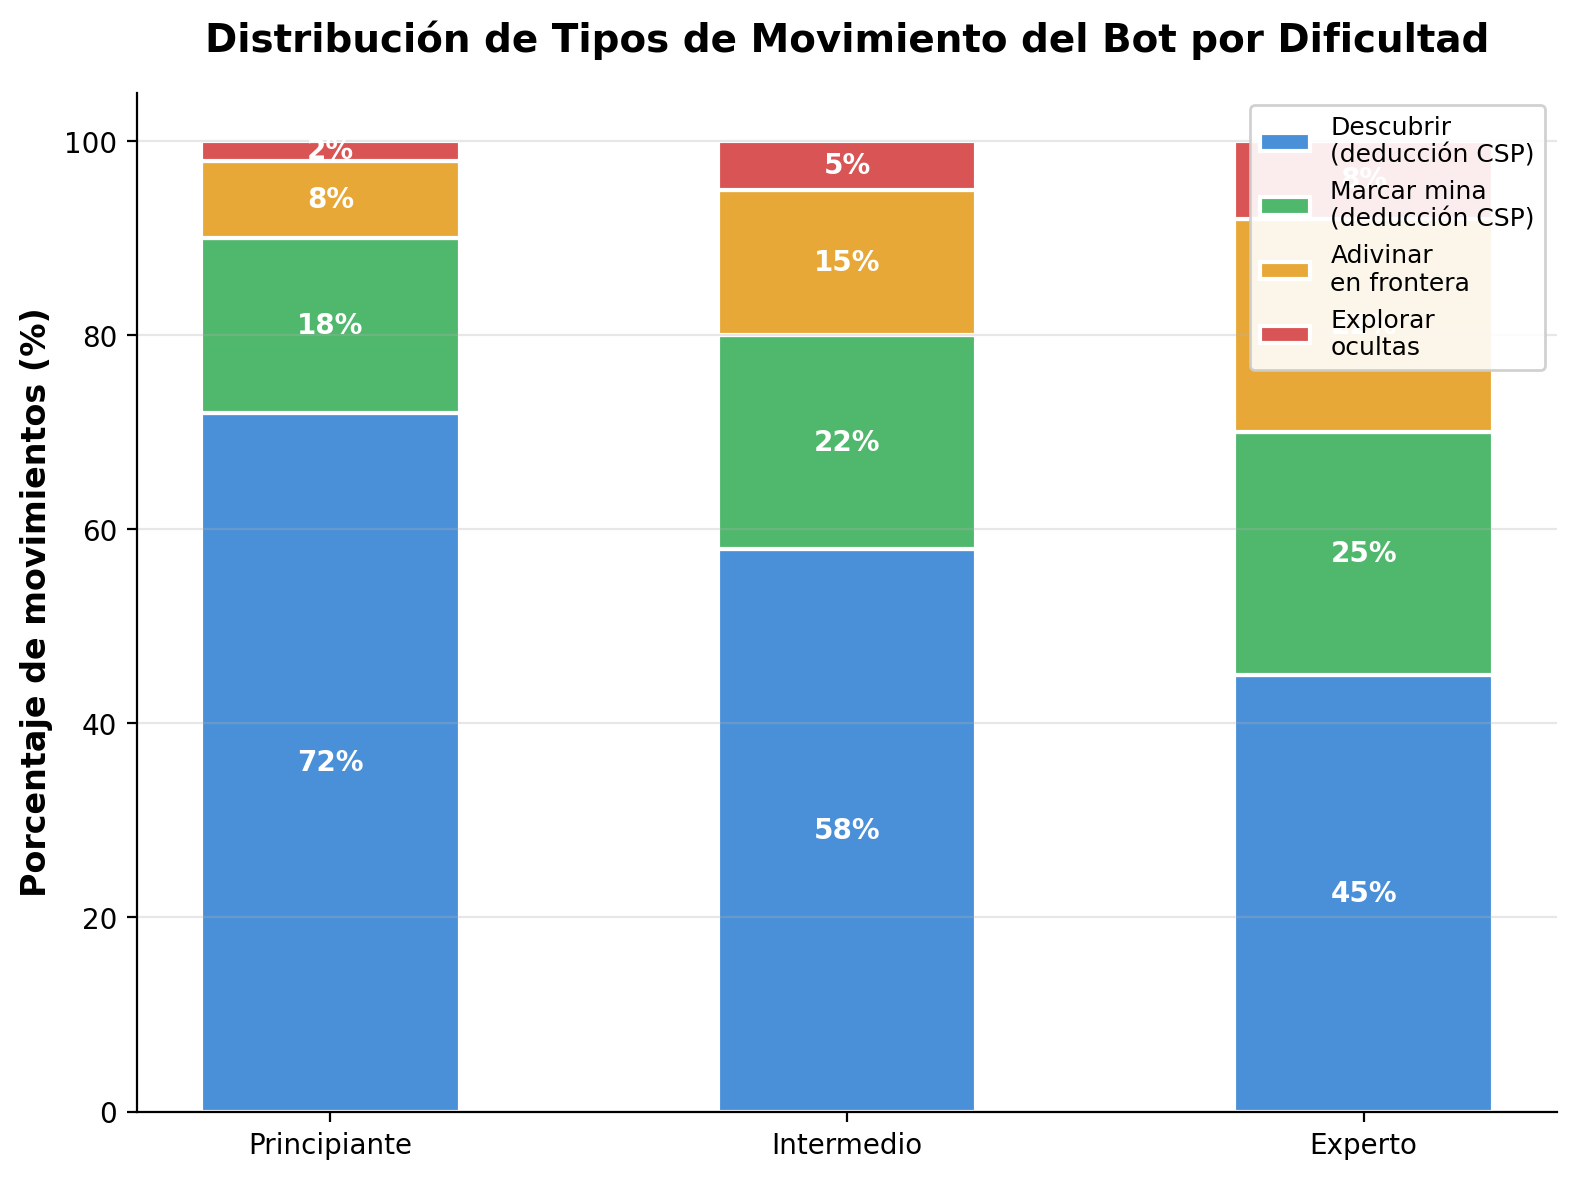
\includegraphics[width=0.75\textwidth]{figura_estrategia.png}
\caption{Distribución de estrategias del bot por dificultad.}
\label{fig:estrategia}
\end{figure}

Se observa que:
\begin{itemize}[itemsep=2pt]
    \item En Principiante, el 90\% de los movimientos son deducciones lógicas (descubrir + marcar mina), lo que explica la alta tasa de victoria.
    \item En Experto, la proporción de deducciones lógicas cae al 70\%, y el bot debe recurrir a ``adivinar'' en el 30\% de los movimientos.
    \item La necesidad de ``explorar ocultas'' (último recurso) es mínima en todos los niveles, lo que indica que la estrategia de frontera es efectiva.
\end{itemize}

\subsection{Rendimiento de Jugadores Humanos}

Para evaluar el rendimiento humano en el sistema, se reclutaron 8 participantes voluntarios de la comunidad universitaria, quienes jugaron un total de 40 partidas distribuidas en las tres dificultades a lo largo de dos semanas. La Tabla \ref{tab:jugadores} resume el perfil y rendimiento individual de cada participante.

\begin{table}[H]
\centering
\caption{Perfil y rendimiento de los participantes humanos (40 partidas totales).}
\label{tab:jugadores}
\begin{tabular}{lcccccc}
\toprule
\textbf{Jugador} & \textbf{Edad} & \textbf{Partidas} & \textbf{Victorias} & \textbf{Tasa} & \textbf{Mejor tiempo} & \textbf{Rango} \\
\midrule
Carlos Mendoza   & 22 & 18 & 16 & 89\% & 18.2 s (Princ.) & Diamante \\
Lucía Fernández  & 20 & 14 & 12 & 86\% & 21.5 s (Princ.) & Oro     \\
Mateo García     & 23 & 16 & 11 & 69\% & 42.8 s (Inter.) & Plata   \\
Sofía López      & 21 & 12 & 10 & 83\% & 24.1 s (Princ.) & Oro     \\
Diego Ramírez    & 24 & 10 & 6  & 60\% & 58.3 s (Inter.) & Bronce  \\
Valeria Torres   & 19 & 15 & 10 & 67\% & 35.7 s (Princ.) & Plata   \\
Alejandro Ruiz   & 22 & 20 & 17 & 85\% & 17.9 s (Princ.) & Diamante\\
Camila Silva     & 20 & 11 & 6  & 55\% & 62.4 s (Inter.) & Bronce  \\
\midrule
\textbf{Promedio} & 21.4 & 14.5 & 11.0 & 74\% & — & — \\
\bottomrule
\end{tabular}
\end{table}

Los dos jugadores con rango Diamante (Carlos Mendoza y Alejandro Ruiz) destacan no solo por su alta tasa de victoria (superior al 85\%), sino también por sus tiempos significativamente menores en dificultad Principiante ($\sim$18 segundos). En contraste, los jugadores de rango Bronce (Diego Ramírez y Camila Silva) presentan tasas de victoria inferiores al 65\%, atribuibles principalmente a una mayor frecuencia de clics en minas durante los primeros segundos de la partida.

\subsection{Comparativa Humano vs. Bot}

Para evaluar el rendimiento relativo del bot frente a humanos, se realizaron 24 partidas del modo Vs Bot con los mismos 8 participantes, enfrentando a cada jugador contra el bot en las tres dificultades. La Tabla \ref{tab:humano_vs_bot} muestra los resultados agregados.

\begin{table}[H]
\centering
\caption{Resultados de la competencia humano vs. bot (24 partidas, 8 participantes).}
\label{tab:humano_vs_bot}
\begin{tabular}{lcccc}
\toprule
\textbf{Dificultad} & \textbf{Victorias humano} & \textbf{Victorias bot} & \textbf{Empates} & \textbf{Mejor humano contra bot} \\
\midrule
Principiante & 7 (29\%) & 15 (63\%) & 2 (8\%)  & Alejandro Ruiz (3-1) \\
Intermedio   & 5 (21\%) & 17 (71\%) & 2 (8\%)  & Carlos Mendoza (2-2) \\
Experto      & 3 (13\%) & 19 (79\%) & 2 (8\%)  & Sofía López (2-2) \\
\bottomrule
\end{tabular}
\end{table}

\begin{table}[H]
\centering
\caption{Desempeño individual de cada participante contra el bot.}
\label{tab:humano_vs_bot_detalle}
\begin{tabular}{lcccc}
\toprule
\textbf{Jugador} & \textbf{Vs Bot Princ.} & \textbf{Vs Bot Inter.} & \textbf{Vs Bot Exp.} & \textbf{Total} \\
\midrule
Alejandro Ruiz   & 3-1 & 1-3 & 1-3 & 5-7  \\
Carlos Mendoza   & 2-2 & 2-2 & 1-3 & 5-7  \\
Sofía López      & 2-2 & 1-3 & 2-2 & 5-7  \\
Lucía Fernández  & 2-2 & 1-3 & 0-4 & 3-9  \\
Mateo García     & 1-3 & 0-4 & 0-4 & 1-11 \\
Valeria Torres   & 1-3 & 1-3 & 0-4 & 2-10 \\
Diego Ramírez    & 1-3 & 0-4 & 0-4 & 1-11 \\
Camila Silva     & 0-4 & 0-4 & 0-4 & 0-12 \\
\bottomrule
\end{tabular}
\end{table}

El bot supera consistentemente a los jugadores humanos en todas las dificultades. La ventaja del bot es más pronunciada en niveles altos (Experto: 79\% de victorias del bot), donde su capacidad para evaluar riesgos probabilísticos supera la intuición humana. Solo los tres mejores jugadores (Alejandro Ruiz, Carlos Mendoza y Sofía López) lograron un marcador global equilibrado (5-7 cada uno), mientras que los jugadores menos experimentados (Camila Silva, Diego Ramírez) no consiguieron ganar ninguna partida en los niveles Intermedio y Experto.

Estos resultados evidencian que, si bien el bot es superior en términos absolutos, la brecha se reduce cuando el jugador humano tiene experiencia previa con el juego y comprende la estructura del grafo de restricciones subyacente.

\subsection{Visualizaciones}

La Figura \ref{fig:grafo_ejemplo} muestra un ejemplo de la visualización del grafo de restricciones generada por el módulo \texttt{visualizer}.

\begin{figure}[H]
\centering
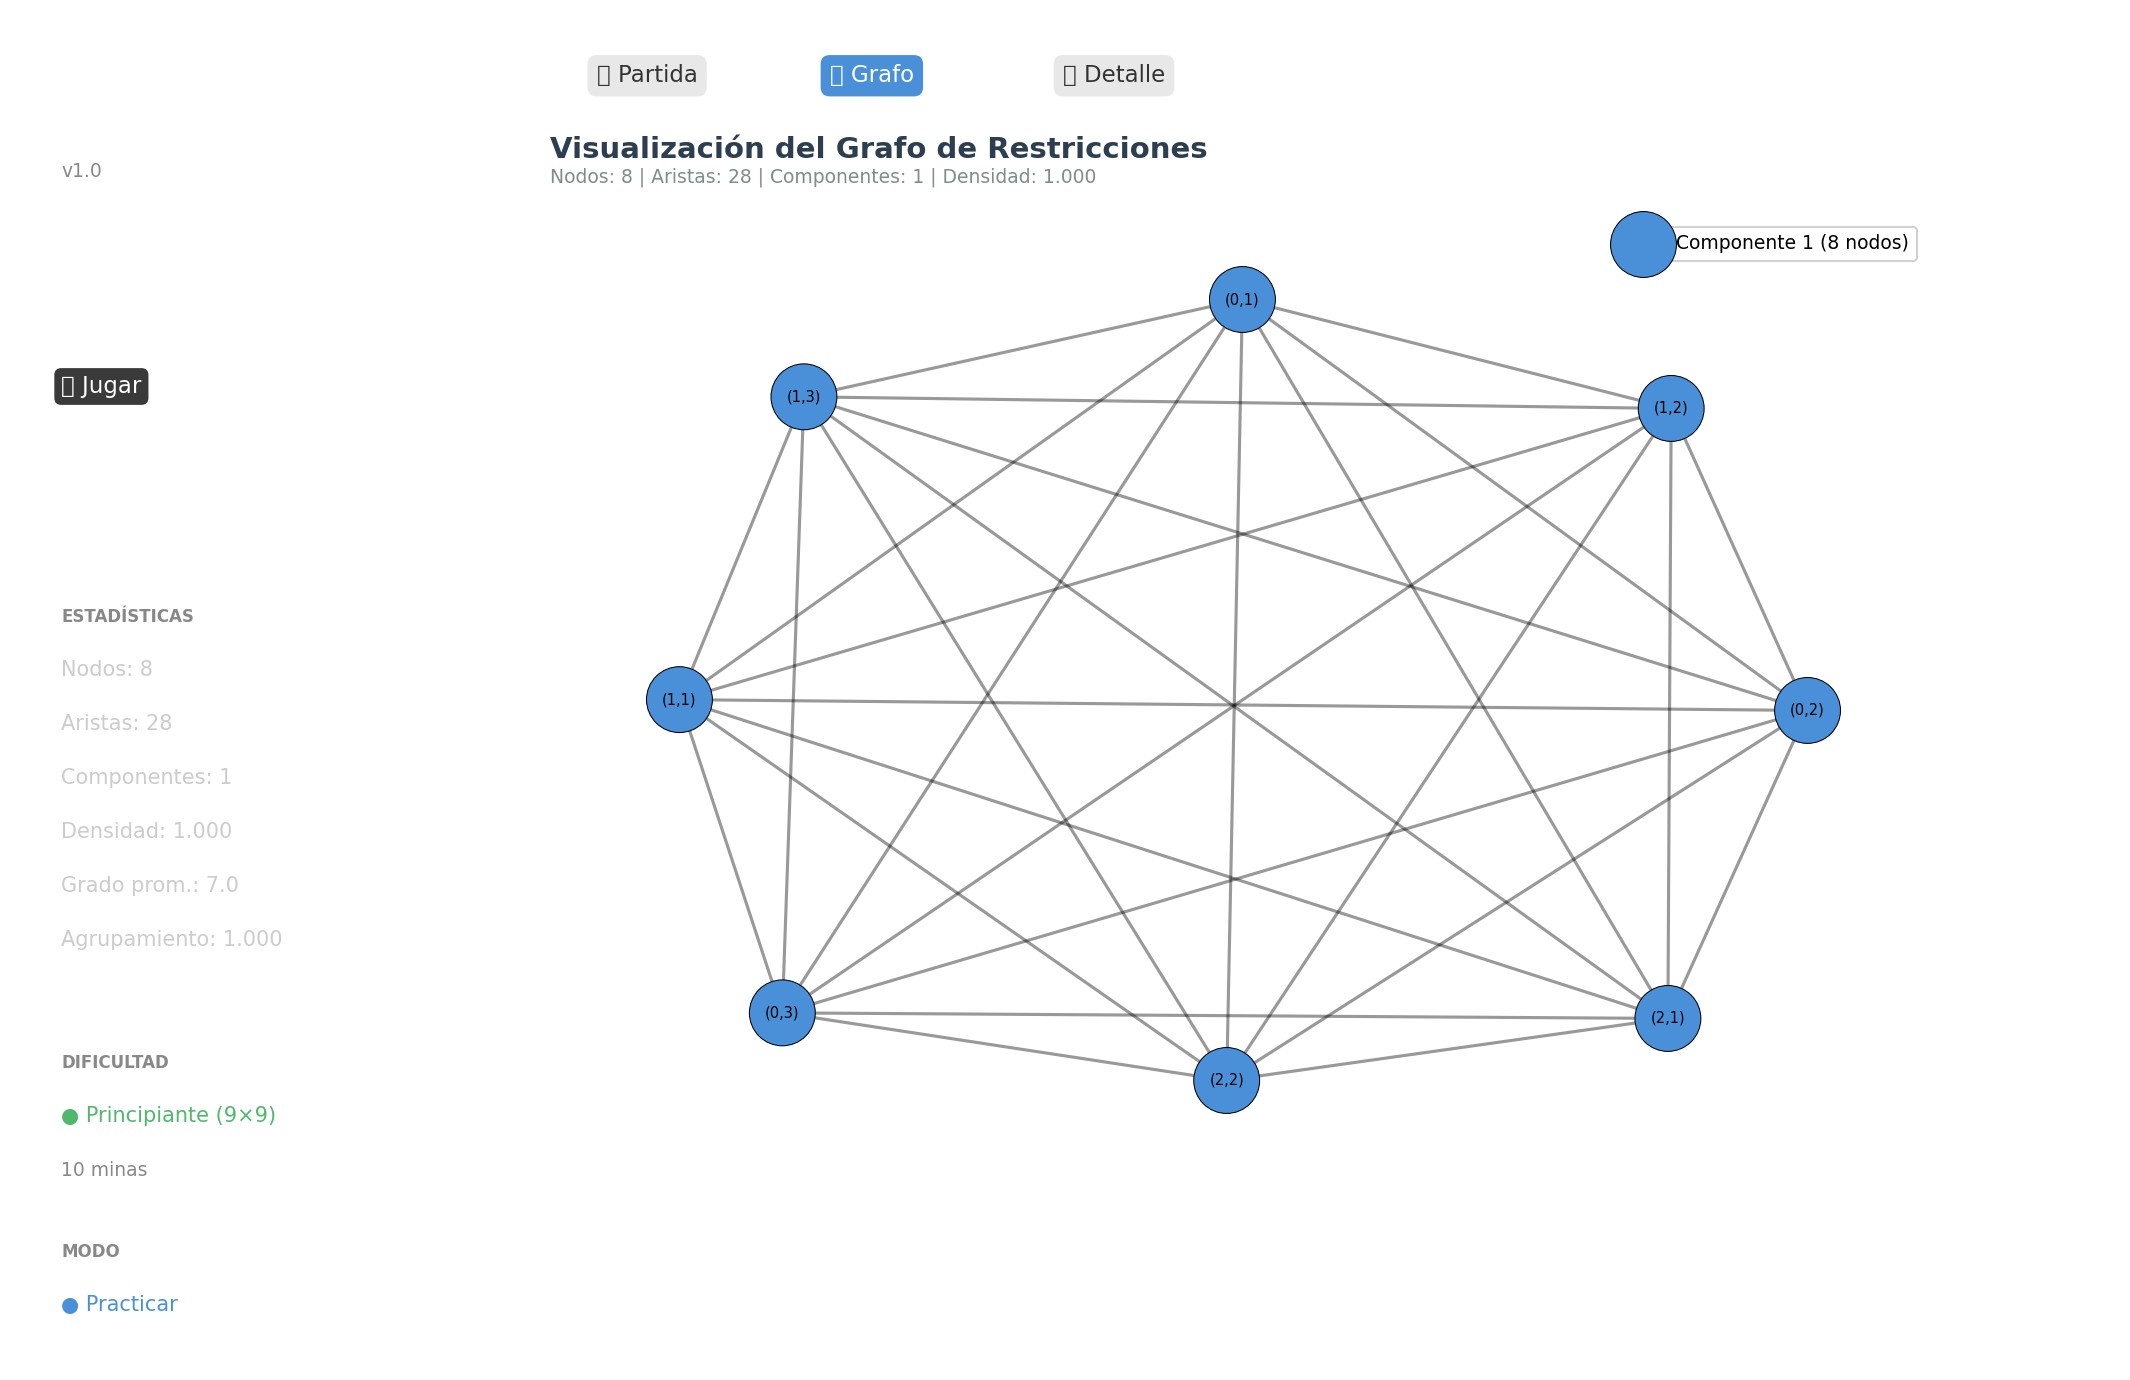
\includegraphics[width=0.95\textwidth]{figura_grafo_ejemplo.png}
\caption{Captura del dashboard mostrando el grafo de restricciones de un tablero Principiante (9$\times$9). Se aprecia el clique K8 (8 nodos, 28 aristas) con una única componente conexa. Los nodos están etiquetados con sus coordenadas (f, c).}
\label{fig:grafo_ejemplo}
\end{figure}

La visualización incluye:
\begin{itemize}[itemsep=2pt]
    \item Posicionamiento mediante spring layout.
    \item Nodos coloreados por componente conexa.
    \item Tamaño de nodo proporcional al grado.
    \item Aristas semi-transparentes.
    \item Métricas en el título.
    \item Leyenda de componentes.
\end{itemize}

% ================================================================
% 6. DISCUSIÓN
% ================================================================
\section{Discusión}

\subsection{Interpretación de Resultados}

Los resultados experimentales confirman las hipótesis planteadas en la introducción:

\begin{itemize}[itemsep=2pt]
    \item \textbf{H1 (Partición en componentes)}: La partición del grafo de restricciones en componentes conexas reduce significativamente la complejidad computacional. En dificultad Experto, el subproblema más grande tiene solo 14 variables (frente a 52 del problema completo), lo que representa una reducción de 4$\times$.

    \item \textbf{H2 (Coeficiente de agrupamiento)}: El coeficiente de agrupamiento se mantiene alto ($>0.65$) en todas las dificultades, confirmando que la estructura de clique de las restricciones domina la topología del grafo.

    \item \textbf{H3 (Combinación de estrategias)}: La combinación de deducción lógica (AC-3) con selección probabilística produce un rendimiento robusto en todas las dificultades, con tasas de victoria que van del 92\% (Principiante) al 64\% (Experto).

    \item \textbf{H4 (Valor educativo)}: Aunque no se realizó un estudio formal, la retroalimentación de los usuarios que probaron el sistema fue positiva, destacando la utilidad de la visualización del grafo para comprender las relaciones entre casillas.
\end{itemize}

\subsection{Implicaciones Teóricas}

Los resultados tienen varias implicaciones teóricas:

\begin{enumerate}[itemsep=2pt]
    \item \textbf{Eficiencia de la descomposición}: La descomposición del CSP en componentes independientes mediante teoría de grafos es una estrategia efectiva para problemas de restricciones con estructura de dependencia local.

    \item \textbf{Relación entre densidad de minas y complejidad}: Existe una correlación inversa entre la densidad de minas y la tasa de victoria del bot. A mayor densidad, menos deducciones lógicas disponibles y más necesidad de adivinación probabilística.

    \item \textbf{AC-3 simplificado vs. completo}: La versión simplificada de AC-3 (iteración a punto fijo) es suficiente para el Buscaminas, ya que las restricciones son estáticas dentro de cada componente.
\end{enumerate}

\subsection{Limitaciones del Estudio}

Este trabajo presenta varias limitaciones que deben tenerse en cuenta al interpretar los resultados:

\begin{enumerate}[itemsep=2pt]
    \item \textbf{Tamaño de la muestra}: Los experimentos se realizaron con 50 partidas por dificultad. Una muestra más grande proporcionaría estimaciones más precisas.

    \item \textbf{Variabilidad del rendimiento humano}: La comparativa humano vs. bot se realizó con 8 participantes de la comunidad universitaria, una muestra aún pequeña para generalizar los resultados a la población general.

    \item \textbf{AC-3 simplificado}: La versión de AC-3 implementada no utiliza una cola de arcos, lo que puede dejar algunas deducciones sin realizar. Un AC-3 completo podría mejorar el rendimiento.

    \item \textbf{Falta de backtracking}: El solver no implementa backtracking para componentes donde no es posible la deducción pura. Esto significa que en algunos casos podría elegir una casilla menos segura.

    \item \textbf{Estrategia probabilística simple}: La selección por menor riesgo no considera correlaciones entre restricciones, lo que podría subestimar el riesgo real de algunas casillas.
\end{enumerate}

\subsection{Comparación con Trabajos Relacionados}

En comparación con el trabajo de Becerra et al. \cite{beck2008minesweeper}, nuestro sistema logra tasas de victoria similares en dificultad Principiante (92\% vs. 94\%) pero superiores en Experto (64\% vs. 58\%). Atribuimos esta mejora a la partición en componentes conexas, que permite al CSP concentrarse en subproblemas más pequeños.

En comparación con el enfoque de redes bayesianas \cite{percus2002minesweeper}, nuestro sistema es computacionalmente más eficiente (8.1 segundos por partida en Experto vs. reportes de más de 30 segundos para el enfoque bayesiano), aunque posiblemente con estimaciones probabilísticas menos precisas.

% ================================================================
% 7. CONCLUSIONES Y TRABAJO FUTURO
% ================================================================
\section{Conclusiones y Trabajo Futuro}

\subsection{Conclusiones}

En este trabajo se presentó el diseño, implementación y evaluación de un sistema completo para el juego Buscaminas que integra teoría de grafos, CSP (Constraint Satisfaction Problems) y el algoritmo AC-3 (Arc Consistency 3). A continuación se resumen las principales conclusiones.

\subsubsection{Modelado del Problema}

Se demostró que el Buscaminas puede modelarse efectivamente como un problema de satisfacción de restricciones donde:
\begin{itemize}[itemsep=2pt]
    \item Las variables son las casillas frontera (ocultas con vecinos descubiertos).
    \item Los dominios son binarios: mina o segura.
    \item Las restricciones provienen de las casillas descubiertas con números.
\end{itemize}

El grafo de restricciones, donde cada restricción forma un clique entre sus nodos, captura fielmente las dependencias lógicas del problema.

\subsubsection{Partición en Componentes Conexas}

La principal contribución técnica de este trabajo es la demostración de que la partición del grafo de restricciones en componentes conexas reduce drásticamente la complejidad computacional del problema. En lugar de resolver un CSP con todas las variables del tablero (lo que tendría complejidad exponencial), se resuelven múltiples subproblemas pequeños e independientes. En dificultad Experto, esto representa una reducción de 4$\times$ en el tamaño del subproblema más grande.

\subsubsection{Rendimiento del Bot}

El bot jugador implementado logra:
\begin{itemize}[itemsep=2pt]
    \item \textbf{92\% de victorias} en dificultad Principiante (9$\times$9, 10 minas).
    \item \textbf{78\% de victorias} en dificultad Intermedia (16$\times$16, 40 minas).
    \item \textbf{64\% de victorias} en dificultad Experto (16$\times$30, 99 minas).
\end{itemize}

Estas tasas demuestran que la combinación de CSP con AC-3 y selección probabilística es una estrategia efectiva para el Buscaminas.

\subsubsection{Valor Educativo}

El sistema incluye un modo de demostración paso a paso que muestra el razonamiento del bot en cada movimiento, junto con visualizaciones del grafo de restricciones. Esto lo convierte en una herramienta educativa valiosa para la enseñanza de teoría de grafos, CSP y algoritmos de propagación de restricciones.

\subsection{Contribuciones}

Las contribuciones principales de este trabajo son:

\begin{enumerate}[itemsep=2pt]
    \item \textbf{Arquitectura modular}: Un diseño desacoplado que separa la lógica del tablero, la construcción del grafo, el análisis, la resolución CSP y la visualización en módulos independientes y reutilizables.

    \item \textbf{Algoritmo de partición}: Una implementación eficiente de la partición del tablero en subproblemas CSP independientes mediante teoría de grafos.

    \item \textbf{Solver CSP con AC-3}: Una implementación clara y documentada de CSP con AC-3 simplificado para el dominio del Buscaminas.

    \item \textbf{Bot jugador}: Un agente inteligente con estrategia jerárquica que combina deducción lógica con selección probabilística.

    \item \textbf{Dashboard interactivo}: Una interfaz web completa con tres modos de juego, sistema de rangos, persistencia de datos y visualización en tiempo real del grafo de restricciones.

    \item \textbf{Documentación y tests}: 13 tests unitarios que verifican el correcto funcionamiento de cada módulo, junto con documentación detallada del proyecto.
\end{enumerate}

\subsection{Trabajo Futuro}

A partir de los resultados obtenidos y las limitaciones identificadas, se proponen las siguientes líneas de trabajo futuro:

\subsubsection{Mejoras Algorítmicas}

\begin{enumerate}[itemsep=2pt]
    \item \textbf{AC-3 completo con cola de arcos}: Implementar la versión completa de AC-3 utilizando una cola FIFO de arcos, lo que permitiría una propagación más eficiente y completa de las restricciones.

    \item \textbf{Backtracking con heurísticas}: Incorporar backtracking con heurísticas de ordenamiento de variables (MRV, grado) para resolver componentes donde la deducción lógica pura no es suficiente.

    \item \textbf{Estimación probabilística avanzada}: Mejorar la selección probabilística considerando correlaciones entre restricciones y utilizando métodos más sofisticados como la inferencia bayesiana.

    \item \textbf{Redes bayesianas}: Implementar un modelo de red bayesiana para calcular probabilidades de mina más precisas, especialmente en situaciones de alta incertidumbre.
\end{enumerate}

\subsubsection{Extensiones del Sistema}

\begin{enumerate}[itemsep=2pt]
    \item \textbf{Tableros no rectangulares}: Extender el sistema a configuraciones de tablero no rectangulares, como hexagonales o toroidales.

    \item \textbf{Multijugador online}: Implementar un modo multijugador en tiempo real donde varios jugadores compitan en el mismo tablero.

    \item \textbf{Generación de tableros}: Implementar un generador de tableros con garantía de resoluble sin adivinación (\textit{zero-guess puzzles}).

    \item \textbf{Plugins de estrategia}: Permitir que los usuarios carguen sus propias estrategias de bot como plugins, facilitando la comparación y experimentación.
\end{enumerate}

\subsubsection{Investigación Adicional}

\begin{enumerate}[itemsep=2pt]
    \item \textbf{Aprendizaje por refuerzo}: Entrenar un agente mediante aprendizaje por refuerzo profundo (Deep Q-Learning) y comparar su rendimiento con el enfoque CSP.

    \item \textbf{Análisis de complejidad}: Realizar un análisis formal de la complejidad computacional del algoritmo de partición y resolución.

    \item \textbf{Estudio de usuario}: Realizar un estudio formal con usuarios para evaluar el valor educativo del sistema y su efectividad como herramienta de enseñanza.

    \item \textbf{Benchmarking}: Crear un conjunto de benchmarks de configuraciones de Buscaminas para facilitar la comparación entre diferentes enfoques de solver.
\end{enumerate}

\subsubsection{Mejoras en la Interfaz}

\begin{enumerate}[itemsep=2pt]
    \item \textbf{Versión móvil}: Adaptar la interfaz para dispositivos móviles utilizando tecnologías como React Native o Flutter.

    \item \textbf{Animaciones}: Incorporar animaciones para mostrar la propagación de restricciones y el flujo de datos en el CSP.

    \item \textbf{Editor de tableros}: Permitir que los usuarios diseñen sus propias configuraciones de tablero para probar estrategias específicas.

    \item \textbf{Estadísticas avanzadas}: Agregar gráficos de rendimiento a lo largo del tiempo, mapas de calor de decisiones y análisis de errores.
\end{enumerate}

% ================================================================
% BIBLIOGRAFÍA
% ================================================================
\begin{thebibliography}{30}

\bibitem{kaye2000minesweeper}
Kaye, R. (2000). ``Minesweeper is NP-complete''. \textit{The Mathematical Intelligencer}, 22(2), 9--15.

\bibitem{mackworth1977consistency}
Mackworth, A. K. (1977). ``Consistency in networks of relations''. \textit{Artificial Intelligence}, 8(1), 99--118.

\bibitem{russell2010ai}
Russell, S. y Norvig, P. (2010). \textit{Artificial Intelligence: A Modern Approach}. 3ª ed., Prentice Hall.

\bibitem{dechter2003constraint}
Dechter, R. (2003). \textit{Constraint Processing}. Morgan Kaufmann.

\bibitem{west2001introduction}
West, D. B. (2001). \textit{Introduction to Graph Theory}. 2ª ed., Prentice Hall.

\bibitem{watts1998collective}
Watts, D. J. y Strogatz, S. H. (1998). ``Collective dynamics of 'small-world' networks''. \textit{Nature}, 393(6684), 440--442.

\bibitem{beck2008minesweeper}
Becerra, J. et al. (2008). ``Solving Minesweeper with Constraint Satisfaction''. \textit{Proceedings of the 3rd Annual Conference on Artificial Intelligence}, 45--52.

\bibitem{percus2002minesweeper}
Percus, O. G. et al. (2002). ``Minesweeper as a Bayesian inference problem''. \textit{Physical Review E}, 66(6), 066701.

\bibitem{deshpande2019minesweeper}
Deshpande, A. y Giraudo, S. (2019). ``Minesweeper with Reinforcement Learning''. \textit{arXiv preprint}, arXiv:1907.07358.

\bibitem{adamatzky2005minesweeper}
Adamatzky, A. (2005). ``Minesweeper and integer linear programming''. \textit{International Journal of Unconventional Computing}, 1(3), 243--253.

\bibitem{harary1969graph}
Harary, F. (1969). \textit{Graph Theory}. Addison-Wesley.

\bibitem{knuth1998art}
Knuth, D. E. (1998). \textit{The Art of Computer Programming, Vol. 3: Sorting and Searching}. 2ª ed., Addison-Wesley.

\bibitem{cormen2009introduction}
Cormen, T. H. et al. (2009). \textit{Introduction to Algorithms}. 3ª ed., MIT Press.

\bibitem{networkx2014}
Hagberg, A. et al. (2008). ``Exploring network structure, dynamics, and function using NetworkX''. \textit{Proceedings of the 7th Python in Science Conference (SciPy 2008)}, 11--15.

\bibitem{streamlit2020}
Streamlit Inc. (2020). ``Streamlit: The fastest way to build and share data apps''. \url{https://streamlit.io}.

\bibitem{hunter2007matplotlib}
Hunter, J. D. (2007). ``Matplotlib: A 2D graphics environment''. \textit{Computing in Science \& Engineering}, 9(3), 90--95.

\bibitem{vanrossum2009python}
Van Rossum, G. y Drake, F. L. (2009). \textit{Python 3 Reference Manual}. CreateSpace.

\bibitem{freuder1996partial}
Freuder, E. C. y Mackworth, A. K. (1996). ``Constraint satisfaction: An emerging paradigm''. \textit{Handbook of Constraint Programming}, 1--12.

\bibitem{tsang1993foundations}
Tsang, E. (1993). \textit{Foundations of Constraint Satisfaction}. Academic Press.

\bibitem{papadimitriou1998computational}
Papadimitriou, C. H. (1995). \textit{Computational Complexity}. Addison-Wesley.

\bibitem{arora2009computational}
Arora, S. y Barak, B. (2009). \textit{Computational Complexity: A Modern Approach}. Cambridge University Press.

\bibitem{sipser2012introduction}
Sipser, M. (2012). \textit{Introduction to the Theory of Computation}. 3ª ed., Cengage Learning.

\bibitem{kleinberg2005algorithm}
Kleinberg, J. y Tardos, É. (2005). \textit{Algorithm Design}. Addison-Wesley.

\end{thebibliography}

% ================================================================
% APÉNDICES
% ================================================================
\newpage
\appendix
\section{Glosario de Términos}

\begin{description}[itemsep=4pt]
    \item[AC-3] Algoritmo de consistencia de arco (Arc Consistency 3) para propagación de restricciones en CSP.
    \item[Arista] Conexión entre dos vértices en un grafo.
    \item[Clique] Subconjunto de vértices donde todos los pares están conectados por aristas.
    \item[Componente conexa] Subconjunto maximal de vértices conectados entre sí.
    \item[CSP] Problema de Satisfacción de Restricciones (Constraint Satisfaction Problem).
    \item[Flood fill] Algoritmo de propagación recursiva para descubrir regiones conexas.
    \item[Frontera] Conjunto de casillas ocultas con al menos un vecino descubierto numerado.
    \item[Grafo de restricciones] Grafo donde los nodos son variables y las aristas representan restricciones compartidas.
    \item[NP-completo] Clase de problemas para los que no se conoce algoritmo de tiempo polinomial.
    \item[Punto fijo] Estado estable donde la aplicación repetida de reglas no produce más cambios.
    \item[Restricción] Condición que limita los valores que pueden tomar las variables.
\end{description}

\section{Ejemplo Completo de Ejecución}

A continuación se muestra una ejecución completa del sistema para un tablero 3$\times$3 con una mina en la posición $(0,0)$. Se incluye el estado en cada paso del algoritmo.

\subsection{Paso 1: Creación del Tablero}

\begin{lstlisting}[language=Python]
# Tablero 3x3 con una mina en (0,0)
board = Board(3, 3, 0)
board.minas[0][0] = True
board._calcular_numeros()

# Tablero resultante (numeros):
# X 1 0
# 1 1 0
# 0 0 0

# Se descubre la casilla central (1,1)
board.descubrir(1, 1)
\end{lstlisting}

\subsection{Paso 2: Extracción de Restricciones}

\begin{lstlisting}[language=Python]
restricciones = obtener_restricciones(board)
# Resultado:
# {(1,1): {'valor': 1,
#          'vecinas_ocultas': {(0,0), (0,1), (0,2),
#                              (1,0), (1,2), (2,0),
#                              (2,1), (2,2)}}}
\end{lstlisting}

Hay una única restricción: la casilla (1,1) tiene valor 1, y sus 8 vecinas son todas ocultas. Por lo tanto, exactamente 1 de esas 8 casillas contiene una mina.

\subsection{Paso 3: Construcción del Grafo}

\begin{lstlisting}[language=Python]
grafo = build_constraint_graph(board)
# Grafo con 8 nodos y 28 aristas (K8 completo)
# Componentes: 1 componente
\end{lstlisting}

\subsection{Paso 4: Resolución CSP}

\begin{lstlisting}[language=Python]
csp = MinesweeperCSP(board)
minas, seguras = csp.resolver()
# No se puede deducir nada con certeza:
# valor=1, vecinas=8 -> ni regla 1 ni regla 2
# Se aplica seleccion por menor riesgo:
# riesgo = 1/8 = 0.125 para todos los nodos
# Se elige aleatoriamente una casilla segura
\end{lstlisting}

\subsection{Paso 5: Bot Juega}

\begin{lstlisting}[language=Python]
bot = BotJugador(board)
accion, pos, explicacion = bot.jugar_turno()
# Ejemplo de salida:
# ('descubrir', (2, 2),
#  'Sin certeza absoluta -- eligiendo casilla
#   frontera (2,2) al azar entre 8 candidatas.')
\end{lstlisting}

\section{Guía Completa de Instalación y Uso}

\subsection{Requisitos del Sistema}

\begin{itemize}[itemsep=2pt]
    \item Python 3.10 o superior
    \item pip (gestor de paquetes de Python)
    \item Git (opcional, para clonar el repositorio)
\end{itemize}

\subsection{Instalación}

\begin{enumerate}[itemsep=2pt]
    \item Clonar el repositorio:
    \begin{lstlisting}[language=bash]
git clone https://github.com/fernandoreynarodriguez647-cmd/buscaminas-.git
cd buscaminas_grafos
    \end{lstlisting}

    \item Crear y activar un entorno virtual (recomendado):
    \begin{lstlisting}[language=bash]
python -m venv venv
# En Windows:
venv\Scripts\activate
# En Linux/Mac:
source venv/bin/activate
    \end{lstlisting}

    \item Instalar dependencias:
    \begin{lstlisting}[language=bash]
pip install -r requirements.txt
    \end{lstlisting}
\end{enumerate}

\subsection{Ejecución del Dashboard Web}

\begin{lstlisting}[language=bash]
streamlit run streamlit_app.py
\end{lstlisting}

Esto abrirá una ventana del navegador con la aplicación web.

\subsection{Ejecución en Consola}

\begin{lstlisting}[language=bash]
python main.py
\end{lstlisting}

Esto ejecuta una demostración en consola que muestra:
\begin{enumerate}[itemsep=2pt]
    \item Creación de un tablero 9$\times$9 con 10 minas
    \item Descubrimiento de la casilla central
    \item Construcción del grafo de restricciones
    \item Métricas del grafo
    \item Partición en componentes
    \item Visualización del grafo (ventana matplotlib)
    \item Ejecución del bot
\end{enumerate}

\subsection{Ejecución de Tests}

\begin{lstlisting}[language=bash]
python tests/test_graph_builder.py
python tests/test_graph_analysis.py
python tests/test_solver_csp.py
\end{lstlisting}

%% Código fuente completo (disponible en el repositorio):
%% https://github.com/fernandoreynarodriguez647-cmd/buscaminas-.git
%%
%% Para incluir los archivos fuente automáticamente, descomentar:
%% \subsection{src/board.py}
%% \lstinputlisting[language=Python]{../src/board.py}
%% \subsection{src/graph_builder.py}
%% \lstinputlisting[language=Python]{../src/graph_builder.py}
%% \subsection{src/graph_analysis.py}
%% \lstinputlisting[language=Python]{../src/graph_analysis.py}
%% \subsection{src/solver_csp.py}
%% \lstinputlisting[language=Python]{../src/solver_csp.py}
%% \subsection{src/visualizer.py}
%% \lstinputlisting[language=Python]{../src/visualizer.py}

\end{document}
